%!TeX program = xelatex
\documentclass[12pt,hyperref,a4paper,UTF8]{ctexart}

\usepackage{UCASReport}
\usepackage{float}
\usepackage{makecell}
\usepackage{enumitem}
\usepackage{booktabs}

\setlist[1]{
    itemsep = 0pt,
    partopsep = 0pt,
    parsep = \parskip,
    topsep = 0pt,
    leftmargin = 2em,
    labelsep = 0.5em
}

\newcommand{\barline}[1]{\overline{#1\rule{0pt}{1.5ex}}}

%%-------------------------------正文开始---------------------------%%
\begin{document}

%%-----------------------封面--------------------%%
\cover

%%------------------摘要-------------%%
%\begin{abstract}
%
%在此填写摘要内容
%
%\end{abstract}

\thispagestyle{empty} % 首页不显示页码

%%--------------------------目录页------------------------%%
\newpage
\thispagestyle{empty}
\tableofcontents
\thispagestyle{empty}


%%------------------------正文页从这里开始-------------------%
\newpage
\setcounter{page}{1}

%%可选择这里也放一个标题
%\begin{center}
%    \title{ \Huge \textbf{{标题}}}
%\end{center}


\section{小组成员分工}

\begin{itemize}
    \item 许XX：论文方法论、阅读分析、撰写方法论部分报告；
    \item 邵XX：负责 VKRayGS 实验复现和扩展、数据生成；
    \item 雷XX：负责分析 VKRayGS 实验结果；
    \item 陈XX：实验结果分析、撰写实验结果部分报告；
    \item Illusionna：汇总组员工作、排版读书报告。
\end{itemize}



\section{引言}
\subsection{研究背景}
三维高斯泼溅（3D Gaussian Splatting, 3DGS）是近年来新视角合成领域的重要方法~\cite{3dgaussiansplatting}。它使用大量显式三维 Gaussian primitive 表示场景，每个 primitive 具有空间位置、形状、颜色和不透明度。相比 NeRF 等隐式神经辐射场方法~\cite{nerf,mipnerf360}，3DGS 更容易映射到高效渲染流程中，因此能够同时获得较好的重建质量和较高的实时渲染效率。

随着 3DGS 被用于数字人、三维重建、动态场景、SLAM、VR/MR 和沉浸式浏览等任务~\cite{hugs,dynamic3dgaussians,splatam}，研究重点逐渐集中到两个方向：一是提升几何一致性和渲染质量，二是进一步提升渲染速度，使其可以满足高分辨率和自由视角交互的帧率需求~\cite{flashgs,lightgaussian,compressed3dgs}。



\subsection{传统 3DGS 的问题}
传统 3DGS 渲染时通常将三维高斯通过局部线性近似投影为图像平面上的二维高斯，然后在屏幕空间进行 splatting~\cite{3dgaussiansplatting}。这种做法速度快，也非常适合硬件光栅化，但其本质依赖局部线性投影。当相机靠近物体、高斯尺度较大、透视变化较强或用户在 VR/MR 中自由移动时，屏幕空间二维椭圆 support 可能无法准确反映真实三维高斯对相机射线的贡献范围，从而产生尖刺、漂浮边缘、局部膨胀、孔洞或 popping artifacts 等几何不一致伪影~\cite{stopthepop,gaussianopacityfields}。



\subsection{RayGS 的动机}
Ray-based Gaussian Splatting，简称 RayGS，通过直接考虑相机射线与三维高斯之间的关系，避免传统 GS 的局部投影近似~\cite{gaussianopacityfields}。对于一个像素射线，RayGS 在三维空间中寻找该射线上高斯密度最大的点，并据此计算不透明度。这样，RayGS 在近距离观察和自由视角移动中通常具有更稳定的几何表现。

但是，RayGS 的直接计算代价较高。已有 RayGS 或 ray casting 形式的 3DGS 方法往往依赖 CUDA 软件渲染或更复杂的 ray tracing 过程~\cite{gaussianopacityfields}，难以在消费级硬件上达到 VR/MR 所需的高帧率。



\subsection{论文核心贡献}
论文 \emph{Hardware-Rasterized Ray-Based Gaussian Splatting}~\cite{hardwarerasterizedraybasedgaussiansplatting} 核心目标是将 RayGS 的高质量和硬件光栅化的高效率结合起来。它的主要贡献可以概括为两点：

\begin{enumerate}
    \item 提出一种硬件光栅化 RayGS renderer。该方法不再在图像平面上直接寻找复杂的 RayGS support，而是在三维空间中为每个 RayGS primitive 构造一个包围 support 的三维 quad，再交给标准 GPU 光栅化管线生成片元，并在 fragment shader 中高效计算 RayGS opacity。
    \item 提出适用于 RayGS 的 MIP 抗混叠方法。该方法从像素中心单射线采样扩展到像素局部面积的平均贡献估计，通过协方差平滑和 opacity modulation 缓解尺度变化导致的 aliasing；这一问题也与 NeRF 和 3DGS 中的多尺度抗混叠研究相关~\cite{mipnerf360,mipsplatting}。
\end{enumerate}



\subsection{报告结构}
本报告按原论文主线组织。第二节介绍 3DGS、RayGS 与 support 等基础；第三节说明传统 GS 如何映射到硬件光栅化；第四节分析论文核心方法 Hardware-Rasterized RayGS；第五节分析 MIP-RayGS；第六节整理论文实验；第七节融合 VKRayGS 仓库复现指南和本地实验结果；第八节进行综合讨论；最后给出结论。



\section{相关工作}
\subsection{3D Gaussian Splatting 的场景表示}
在 3DGS 中，一个场景被表示为一组三维 Gaussian primitive~\cite{3dgaussiansplatting}：
\begin{equation}
\displaystyle
S := \left\{ \left(\mu_i, \Sigma_i, o_i, \xi_i\right) \right\}_{i=1}^{N}.
\end{equation}

其中，第 $i$ 个 primitive 包含：

\begin{itemize}
    \item $\mu_i \in \mathbb{R}^3$：高斯中心位置；
    \item $\Sigma_i \in \mathbb{R}^{3\times 3}$：协方差矩阵，描述高斯尺度、形状和方向；
    \item $o_i \in [0,1]$：先验不透明度；
    \item $\xi_i \in \mathbb{R}^d$：特征向量，通常可理解为颜色或球谐颜色系数。
\end{itemize}

协方差矩阵通常可以分解为旋转和尺度：
\begin{equation}
\displaystyle
\Sigma_i = R_i S_i^2 R_i^\top ,
\end{equation}

其中 $R_i$ 表示高斯主轴方向，$S_i$ 表示三个主方向上的尺度。因此，一个 Gaussian primitive 可以直观理解为三维空间中带颜色和透明度的椭球状半透明云团。



\subsection{3DGS 的渲染公式与 alpha blending}
对于一个像素，其对应一条从相机中心出发的射线 $x$。渲染结果由多个 Gaussian primitive 按照深度顺序进行 alpha blending 得到：
\begin{equation}
\displaystyle
R(x;S)
=
\sum_{i=1}^{N}
\xi_{\nu_i}\,
\omega_{\nu_i}(x;S)
\prod_{j=1}^{i-1}
\left[1-\omega_{\nu_j}(x;S)\right].
\end{equation}

其中，$\nu$ 表示与当前相机和射线相关的 primitive 排序，通常按照深度由近到远排列；$\omega_i(x;S)$ 表示第 $i$ 个 primitive 对当前射线的不透明度。

不透明度写为：
\begin{equation}
\displaystyle
\omega_i(x;S)
=
o_i \exp\!\left(
-\frac{1}{2}D(x;\mu_i,\Sigma_i)
\right).
\end{equation}

这里 $D(x;\mu_i,\Sigma_i)$ 是当前像素射线与该高斯之间的 divergence 或距离度量。该值越小，说明射线越接近高斯核心区域，primitive 对像素贡献越大；该值越大，则贡献越小。传统 GS 与 RayGS 的核心区别就在于 $D$ 的定义不同。



\subsection{Primitive support 与截断阈值}
由于高斯分布理论上具有无限支撑，实际渲染中需要设定最小不透明度阈值 $p_{\min}$，将贡献过小的区域忽略。对于一个 primitive，当其不透明度大于等于该阈值时，认为该射线位于该 primitive 的 support 内。

由不透明度公式可得 support 条件：
\begin{equation}
\displaystyle
D(x;\mu,\Sigma) \leq \kappa ,
\qquad
\kappa
=
-2\log\!\left(\frac{p_{\min}}{o}\right).
\end{equation}

当 $D(x;\mu,\Sigma)=\kappa$ 时，对应 support 的边界。support 的意义是限定一个高斯实际需要参与渲染的像素或射线范围，从而避免对整张图像做无意义计算。



\subsection{传统 GS 的屏幕空间投影}
传统 GS 首先通过相机投影函数 $\pi(\cdot)$ 将三维点映射到图像平面~\cite{3dgaussiansplatting}。其 divergence 定义为：
\begin{equation}
\displaystyle
D_{\mathrm{gs}}(x;\mu,\Sigma)
=
\left(\pi(x)-\pi(\mu)\right)^\top
\Sigma_{\pi}^{-1}
\left(\pi(x)-\pi(\mu)\right),
\end{equation}

其中二维协方差矩阵由局部线性化得到：
\begin{equation}
\displaystyle
\Sigma_{\pi}
=
J_{\pi}\Sigma J_{\pi}^{\top}.
\end{equation}

$J_{\pi}$ 是投影函数 $\pi$ 在高斯中心 $\mu$ 处的雅可比矩阵。该公式表示传统 GS 在 $\mu$ 附近对透视投影进行局部线性化，将三维协方差 $\Sigma$ 近似变换为图像平面中的二维协方差 $\Sigma_{\pi}$。因此，传统 GS 本质上是在图像平面上计算像素位置与二维投影高斯之间的马氏距离。

该方法的优点是 support 在图像平面上形成二维椭圆，容易用一个 quad 包围，并交给 GPU 光栅化器处理。局限则是局部线性近似在近景、强透视和大尺度 Gaussian 下容易破坏几何一致性。



\subsection{Ray-Based Gaussian Splatting}
RayGS 放弃传统 GS 中的二维投影近似，转而直接考虑相机射线与三维高斯之间的关系~\cite{gaussianopacityfields}。对于像素射线 $x$，RayGS 寻找该射线上高斯密度最大的点 $\tau(x)x$，并根据该点与高斯中心之间的马氏距离计算不透明度。RayGS divergence 为：
\begin{equation}
\displaystyle
D_{\mathrm{ray}}(x;\mu,\Sigma)
=
\left(\tau(x)x-\mu\right)^\top
\Sigma^{-1}
\left(\tau(x)x-\mu\right),
\end{equation}

其中：
\begin{equation}
\displaystyle
\tau(x)
=
\frac{x^\top \Sigma^{-1}\mu}
{x^\top \Sigma^{-1}x}.
\end{equation}

几何上，$\tau(x)x$ 表示射线 $x$ 上高斯密度最大的点。若该点接近高斯中心，则当前射线穿过高斯核心区域；若该点远离高斯中心，则高斯贡献较小。

RayGS 的优势是几何一致性更好，可以减少传统 GS 在近距离观察时可能出现的尖刺、错位和 popping artifacts。它的问题是 support 不再天然对应图像平面中的简单二维椭圆，而是由一组相机射线定义。因此，RayGS 不能直接套用传统 GS 的屏幕空间 quad 光栅化方案。



\section{传统 GS 的硬件光栅化流程}
\subsection{传统 GS 容易硬件光栅化}
传统 GS 之所以渲染速度快，是因为它能够自然映射到标准 GPU 光栅化管线中~\cite{3dgaussiansplatting,vkgs}。基本流程如下：

\begin{enumerate}
    \item 将三维高斯投影到图像平面，得到二维高斯；
    \item 该二维高斯的 support 是图像平面中的二维椭圆；
    \item 使用一个 quad 包围该椭圆；
    \item GPU 光栅化器确定该 quad 覆盖的像素；
    \item fragment shader 在 quad 覆盖的片元处计算不透明度；
    \item 多个 primitive 按深度顺序通过 alpha blending 合成最终颜色。
\end{enumerate}



\subsection{Vertex shader：由二维椭圆构造 quad}
在传统硬件光栅化 GS 中，vertex shader 负责构造包围二维椭圆 support 的 quad。对二维协方差矩阵进行特征分解：
\begin{equation}
\displaystyle
\Sigma_{\pi}
=
U_{\mathrm{gs}}\Lambda_{\mathrm{gs}}U_{\mathrm{gs}}^\top ,
\end{equation}

其中 $U_{\mathrm{gs}}$ 表示椭圆主轴方向，$\Lambda_{\mathrm{gs}}$ 表示主轴尺度。由此可以从标准正方形出发，通过缩放、旋转和平移得到图像平面中的 quad 顶点：
\begin{equation}
\displaystyle
V_{\mathrm{gs}}
=
T_{\mathrm{gs}}H(Z_{\mathrm{gs}}).
\end{equation}

$Z_{\mathrm{gs}}$ 表示标准 quad 的局部坐标，$T_{\mathrm{gs}}$ 表示将标准 quad 变换到图像平面中目标位置和形状的变换矩阵。



\subsection{Fragment shader：插值坐标与不透明度计算}
fragment shader 的任务是计算 quad 内每个像素处的 divergence 和不透明度。传统 GS 利用 GPU 的顶点属性插值能力，使片元阶段不需要重新计算完整二维马氏距离。对于 quad 内任意片元，可通过插值得到局部坐标，并计算：
\begin{equation}
\displaystyle
D_{\mathrm{gs}}
=
\left\| Z_{\mathrm{gs}}\alpha \right\|^2 ,
\end{equation}

其中 $\alpha$ 表示片元相对于 quad 顶点的插值系数。随后将 $D_{\mathrm{gs}}$ 代入不透明度公式，得到该 primitive 对当前像素的 alpha 值。

这一流程说明，传统 GS 的高效性来自两个方面：quad 限定了需要计算的局部像素范围；fragment shader 只需执行插值、点积和指数运算等较简单操作。



\subsection{传统流程的局限}
传统 GS 的 quad 位于图像平面，其有效性依赖二维椭圆 support。但 RayGS 的 support 由三维射线关系定义，在图像平面上可能不再是简单椭圆。如果仍然直接使用传统 GS 的屏幕空间投影近似，就会丢失 RayGS 改善几何一致性的意义。因此，本文需要为 RayGS 设计新的硬件光栅化几何代理，而不能直接用于 RayGS。



\section{论文方法：Hardware-Rasterized RayGS}
\subsection{总体思想}
本文的核心问题是：如何将 RayGS 组织成类似传统 GS 的“quad + shader + blending”硬件光栅化流程？

传统 GS 的 quad 位于图像平面中，因为其 support 是二维椭圆；而 RayGS 的 support 由射线定义。本文提出的关键思想是：不必在图像平面中直接寻找 RayGS support 的复杂形状，而是在三维空间中构造一个 quad。只要该三维 quad 能够与该 primitive support 中所有需要计算贡献的相机射线相交，它就可以作为这个 primitive 的光栅化代理。GPU 将该三维 quad 投影到屏幕后，即可自动生成需要处理的片元。



\subsection{RayGS support 边界的几何分析}
对于一个 RayGS primitive，考虑所有位于 support 边界上的相机射线：
\begin{equation}
\displaystyle
D_{\mathrm{ray}}(x;\mu,\Sigma)=\kappa .
\end{equation}

对每条边界射线，取其最大高斯密度点 $\tau(x)x$。这些点组成集合：
\begin{equation}
\displaystyle
E
=
\left\{
\tau(x)x \;\middle|\;
D_{\mathrm{ray}}(x;\mu,\Sigma)=\kappa,\;
x\in\mathbb{R}^{3}\setminus\{0\}
\right\}.
\end{equation}

$E$ 表示所有 support 边界射线上的最大密度点。论文证明，该集合实际上是嵌入三维空间中的一个二维椭圆。

其几何直觉是：通过对原始三维高斯进行旋转、尺度归一化和方向对齐，可以将该集合映射到单位球面上固定高度的圆。由于该映射可逆，原空间中的 $E$ 就是单位圆经过反向线性变换得到的三维椭圆。这个结论非常关键：虽然 RayGS 的屏幕空间 support 可能复杂，但边界射线上的最大密度点在三维空间中具有规整椭圆结构，因此可以用三维 quad 包围。


\subsection{Vertex shader：三维 quad 构造}
在确定 $E$ 是三维椭圆后，下一步是在 vertex shader 中构造包围该椭圆的三维 quad。由于 $E$ 与二维单位圆 $S^1$ 存在可逆映射，本文先在单位圆空间中构造包围四边形，再通过反向映射将其变换回三维空间。

理论上，包围单位圆的 quad 有无穷多个，映射回三维空间后也会得到无穷多个有效 quad。但这些 quad 投影到屏幕后的面积不同，导致 fragment shader 需要处理的像素数量不同。理想情况下应选择投影面积最小的 quad，但直接优化屏幕投影面积会增加 vertex shader 复杂度。因此，本文采用折中方案：在三维空间中构造与椭圆主轴对齐的紧致矩形。

具体而言，作者在单位圆上寻找一点 $u_1$，使其经过反向映射 $\Phi^{-1}$ 到三维椭圆后，距离椭圆中心最远：
\begin{equation}
\displaystyle
u_1
\in
\arg\max_{u\in S^1}
\left\|
\Phi^{-1}(u)-\Phi^{-1}(0)
\right\|^2 .
\end{equation}

该问题可以化为二维二次型最大化：
\begin{equation}
\displaystyle
u_1
\in
\arg\max_{u\in S^1}
u^\top B u ,
\end{equation}

其中 $B$ 是一个 $2\times 2$ 矩阵。于是 $u_1$ 可以通过最大特征值对应的特征向量求得，与其正交的方向 $u_0$ 对应椭圆短轴方向。组合得到：
\begin{equation}
\displaystyle
U_{\mathrm{ray}}
=
\left(u_0,u_1\right).
\end{equation}

最终 RayGS 的三维 quad 顶点可写成与传统 GS 类似的形式：
\begin{equation}
\displaystyle
V_{\mathrm{ray}}
=
T_{\mathrm{ray}}H(Z_{\mathrm{ray}}),
\end{equation}

其中：
\begin{equation}
\displaystyle
Z_{\mathrm{ray}}
=
\frac{\sqrt{\kappa}}{b}O,
\qquad
T_{\mathrm{ray}}
=
\left[
Q_{0:2}U_{\mathrm{ray}}
\quad
\mu
\right].
\end{equation}

这里 $O$ 表示标准正方形的四个顶点，$Z_{\mathrm{ray}}$ 表示缩放后的标准 quad 坐标，$U_{\mathrm{ray}}$ 使 quad 与三维椭圆主轴对齐，$T_{\mathrm{ray}}$ 将其变换到三维空间中的正确位置。该构造与传统 GS 的 $V_{\mathrm{gs}}=T_{\mathrm{gs}}H(Z_{\mathrm{gs}})$ 形成清晰对应：传统 GS 的 quad 位于图像平面，RayGS 的 quad 位于三维空间。


\subsection{Fragment shader：快速计算 RayGS divergence}
完成三维 quad 构造后，GPU 光栅化器会将其投影到屏幕并生成片元。对于每个片元，fragment shader 需要计算 RayGS divergence：
\begin{equation}
\displaystyle
D_{\mathrm{ray}}(x;\mu,\Sigma).
\end{equation}

如果直接按照 RayGS 原始定义计算，就需要对每个像素重新求最大密度点 $\tau(x)x$，代价较高。本文证明，通过 vertex shader 传入的 $Z_{\mathrm{ray}}$ 并利用硬件插值，可以快速恢复 $D_{\mathrm{ray}}$。对于 quad 内任意片元，设其插值系数为 $\alpha$，则：
\begin{equation}
\displaystyle
D_{\mathrm{ray}}(V_{\mathrm{ray}}\alpha;\mu,\Sigma)
=
\left(
c^{-2}
+
\left\|Z_{\mathrm{ray}}\alpha\right\|^{-2}
\right)^{-1}.
\end{equation}

这意味着 fragment shader 不需要重新执行完整 ray-Gaussian 最大密度点计算，只需要利用插值得到的 $Z_{\mathrm{ray}}\alpha$，计算向量长度和简单标量函数，即可得到 RayGS divergence。随后代入不透明度公式：
\begin{equation}
\displaystyle
\omega(x)
=
o\exp\!\left(
-\frac{1}{2}D_{\mathrm{ray}}(x;\mu,\Sigma)
\right),
\end{equation}

最终通过标准 alpha blending 合成图像。



\subsection{方法小结}
Hardware-Rasterized RayGS 的流程可以概括为：

\begin{enumerate}
    \item 分析 RayGS primitive 的 support 边界；
    \item 取边界射线上的最大密度点，得到集合 $E$；
    \item 证明 $E$ 是三维空间中的二维椭圆；
    \item 构造包围该椭圆的三维 quad；
    \item 由 GPU 光栅化器生成覆盖片元；
    \item 在 fragment shader 中利用插值快速计算 $D_{\mathrm{ray}}$；
    \item 计算不透明度并通过 alpha blending 合成。
\end{enumerate}

该方法没有简单地把 RayGS 近似回传统 GS，而是在保持 RayGS divergence 形式的基础上，为其重新设计了适合 GPU 光栅化管线的几何代理和片元计算方式。因此，它兼顾 RayGS 的高质量和传统硬件光栅化的高效率。



\section{RayGS 的 MIP 抗混叠方法}

\subsection{MIP 问题来源：像素中心射线采样的不足}
虽然 RayGS 改善了传统 GS 的几何一致性问题，但它仍然面临采样尺度问题。标准渲染通常使用像素中心的一条相机射线代表整个像素区域。然而，一个像素实际对应屏幕上的一小块面积。当某个 Gaussian primitive 在屏幕上小于一个像素时，单条中心射线采样会带来明显误差。

例如，如果像素中心射线恰好穿过该高斯，整个像素就可能被赋予该高斯颜色；如果中心射线没有穿过，则该像素可能完全不受该高斯影响。真实情况应是该高斯只覆盖像素的一部分，最终颜色应该按覆盖面积与背景混合。这种单点采样不足会造成 aliasing，表现为锯齿、闪烁、远处细线断裂或小物体忽隐忽现。



\subsection{从单射线采样到像素面积平均}
本文提出适用于 RayGS 的 MIP 处理方法。其核心思想是从像素中心单射线采样扩展为对像素局部面积的平均贡献估计。类似的尺度采样思想在 Mip-NeRF 360 和 Mip-Splatting 中也被用于缓解多尺度渲染混叠~\cite{mipnerf360,mipsplatting}。

对于归一化相机射线 $x$，RayGS 首先找到射线上高斯密度最大的点 $\tau(x)x$。随后在该点处构造一个与射线 $x$ 垂直的局部平面，将三维高斯分布边缘化到该二维平面上，得到平面中的二维高斯。再使用适当大小的各向同性二维高斯进行平滑，以近似高斯在像素面积上的积分。

直观上，这相当于不再用一根无限细的射线判断像素是否命中高斯，而是估计高斯对像素对应小区域的平均影响。



\subsection{协方差平滑与近似 MIP 公式}
论文推导得到的 MIP 后分布形式，可以理解为将原始协方差 $\Sigma$ 替换为带平滑项的协方差：
\begin{equation}
\displaystyle
\hat{\Sigma}_{x}
=
\Sigma
+
\frac{\sigma_x^2}{\tau(x)^2}I .
\end{equation}

其中，$\sigma_x^2$ 表示沿射线单位距离处的像素面积。像素对应的空间面积越大，需要的平滑越强。

但是，理论上的 $\hat{\Sigma}_x$ 依赖具体像素射线 $x$，若直接使用会增加 fragment shader 负担。因此，本文引入近似：将 $\sigma_x$ 视为常量，得到像素无关的平滑协方差 $\hat{\Sigma}$；同时用 primitive 级别代表值近似 modulation factor 中的射线相关项。最终近似 MIP-RayGS 不透明度为：
\begin{equation}
\displaystyle
\omega^{\mathrm{mip}}(x)
\approx
o_i
\sqrt{
\frac{|\Sigma|c^2}
{|\hat{\Sigma}|\hat{c}^{\,2}}
}
\exp\!\left(
-\frac{1}{2}
D_{\mathrm{ray}}(x;\mu,\hat{\Sigma})
\right).
\end{equation}

该公式包含两部分。指数项使用平滑后的协方差 $\hat{\Sigma}$，相当于根据像素尺度对高斯进行滤波；前面的平方根项是 opacity modulation，用于修正平滑后整体不透明度的变化。



\subsection{Opacity modulation 的必要性}
如果只平滑协方差而不调整 opacity，高斯会变得更宽，可能导致物体异常变粗或变亮。论文图 4 中自行车远景结果显示，不使用 opacity modulation 时，虽然 aliasing 得到缓解，但自行车轮辐等细结构会显得不自然地变粗。因此，完整 MIP 公式既要对协方差进行平滑，也要通过 opacity modulation 保持整体不透明度一致，从而在减少锯齿和闪烁的同时避免形状膨胀伪影。



\subsection{MIP-RayGS 与 MSAA 的区别}
MIP-RayGS 和 MSAA 都与抗混叠有关，但侧重点不同。MSAA 通过多重采样改善轮廓采样质量，通常会显著增加片元处理和显存带宽开销；MIP-RayGS 则从 primitive 分布和像素尺度出发，在 RayGS opacity 计算中引入尺度相关滤波，适合缓解远景高频结构的闪烁和锯齿~\cite{mipsplatting}。论文图 4 表明，4x MSAA 能改善 aliasing 但成本更高，而完整 MIP formulation 可以在较小开销下获得更稳定的视觉效果。



\section{论文实验设计与结果分析}
\subsection{实验目标与评价问题}
论文实验的主要目标是验证 VKRayGS 是否能在保持 RayGS 渲染质量的同时，通过 Vulkan 硬件光栅化显著提升渲染速度。需要注意，该对比不是简单比较普通 3DGS 与 RayGS，而是比较 RayGS 路线下的 CUDA renderer 和 Vulkan 硬件光栅化 renderer。



\subsection{数据集与评价协议}
论文使用 MipNeRF360 和 Tanks\&Temples 数据集~\cite{mipnerf360,tanksandtemples}。MipNeRF360 包含 bicycle、bonsai、counter、flowers、garden、kitchen、room、stump、treehill 等场景；Tanks\&Temples 包含 barn、caterpillar、ignatius、meetingroom、truck 等场景。评价时每隔 8 张图取 1 张作为测试集，并在同一批测试视角上统计质量指标和 FPS。

指标包括：

\begin{itemize}
    \item FPS：渲染速度，越高越好；
    \item PSNR：像素级重建质量，越高越好；
    \item SSIM：结构相似度，越高越好；
    \item LPIPS：感知差异，越低越好。
\end{itemize}

论文主实验硬件为 RTX2080。定量实验中 MIP 关闭，因为来自 GOF 的模型已经包含相关协方差处理~\cite{gaussianopacityfields}；MIP 的作用主要通过定性图展示。



\subsection{对比方法}

\begin{table}[H]
    \centering
    \caption{论文实验对象与对比方法}
    \setlength{\tabcolsep}{0pt}
    \renewcommand{\arraystretch}{1.2}
    \begin{tabular}{cccc}
        \bottomrule[1.5pt]
        \textbf{方法} & \textbf{含义} & \textbf{实现方式} & \textbf{作用} \\
        \midrule[0.5pt]
        GOF & Gaussian Opacity Field~\cite{gaussianopacityfields} & CUDA renderer & 主要 baseline \\
        VKRayGS & 本文方法 & Vulkan 硬件光栅化 renderer & 主方法 \\
        VKGS & Vulkan 版普通 3DGS renderer~\cite{vkgs} & Vulkan & 本文实现基础 \\
        GS & 普通 3D Gaussian Splatting~\cite{3dgaussiansplatting} & CUDA / 软件光栅化 & 背景对照 \\
        \toprule[1.5pt]
    \end{tabular}
\end{table}



\subsection{定量结果：速度提升与质量保持}
论文表 1 显示，VKRayGS 在 RTX2080 上将 GOF 的个位数 FPS 提升到百级 FPS，平均约 40$\times$ 加速。表~\ref{tab:paper_fps} 整理了每个场景的 FPS 和提升倍数。

\begin{table}[H]
    \centering
    \caption{论文定量结果：FPS 与提升倍数}
    \label{tab:paper_fps}
    \setlength{\tabcolsep}{2.5pt}
    \renewcommand{\arraystretch}{1.15}
    \begin{tabular}{cccccc}
        \bottomrule[1.5pt]
        \textbf{Scene} & \textbf{Dataset} & \textbf{N / M} & \textbf{GOF FPS} & \textbf{VKRayGS FPS} & \textbf{提升倍数} \\
        \midrule[0.5pt]
        bicycle & MipNeRF360 & 5.35 & 4 & 177 & 44.25$\times$ \\
        bonsai & MipNeRF360 & 1.07 & 6 & 341 & 56.83$\times$ \\
        counter & MipNeRF360 & 0.82 & 6 & 292 & 48.67$\times$ \\
        flowers & MipNeRF360 & 3.28 & 6 & 191 & 31.83$\times$ \\
        garden & MipNeRF360 & 4.40 & 4 & 172 & 43.00$\times$ \\
        kitchen & MipNeRF360 & 1.07 & 5 & 242 & 48.40$\times$ \\
        room & MipNeRF360 & 1.09 & 5 & 305 & 61.00$\times$ \\
        stump & MipNeRF360 & 4.97 & 6 & 186 & 31.00$\times$ \\
        treehill & MipNeRF360 & 4.02 & 5 & 184 & 36.80$\times$ \\
        barn & Tanks\&Temples & 0.83 & 10 & 312 & 31.20$\times$ \\
        caterpillar & Tanks\&Temples & 1.43 & 7 & 247 & 35.29$\times$ \\
        ignatius & Tanks\&Temples & 2.60 & 7 & 203 & 29.00$\times$ \\
        meetingroom & Tanks\&Temples & 0.95 & 7 & 351 & 50.14$\times$ \\
        truck & Tanks\&Temples & 2.14 & 7 & 195 & 27.86$\times$ \\
        \toprule[1.5pt]
    \end{tabular}
\end{table}

质量指标方面，VKRayGS 的 PSNR 和 SSIM 多数略低于 GOF，但差距通常不大；LPIPS 在 bicycle、bonsai、room、truck 等场景中反而更好。表~\ref{tab:paper_quality_delta} 给出 VKRayGS 相对 GOF 的质量差值，其中 LPIPS 越低越好。

\begin{table}[H]
    \centering
    \caption{论文定量结果：质量指标差值（VKRayGS - GOF；LPIPS 越低越好）}
    \label{tab:paper_quality_delta}
    \setlength{\tabcolsep}{20pt}
    \renewcommand{\arraystretch}{1.15}
    \begin{tabular}{cccc}
        \bottomrule[1.5pt]
        \textbf{Scene} & \textbf{PSNR $\Delta$} & \textbf{SSIM $\Delta$} & \textbf{LPIPS $\Delta$} \\
        \midrule[0.5pt]
        bicycle & -0.16 & +0.000 & -0.003 \\
        bonsai & -0.14 & -0.007 & -0.036 \\
        counter & -0.12 & -0.005 & -0.028 \\
        flowers & -0.06 & -0.001 & +0.001 \\
        garden & -0.12 & -0.001 & -0.005 \\
        kitchen & -0.11 & -0.004 & -0.015 \\
        room & -0.26 & -0.009 & -0.036 \\
        stump & -0.02 & +0.002 & -0.003 \\
        treehill & +0.08 & -0.002 & +0.001 \\
        barn & -0.69 & -0.009 & +0.002 \\
        caterpillar & -0.56 & -0.010 & +0.005 \\
        ignatius & -0.34 & -0.011 & +0.002 \\
        meetingroom & -0.79 & -0.014 & -0.005 \\
        truck & -0.50 & -0.011 & -0.012 \\
        \toprule[1.5pt]
    \end{tabular}
\end{table}

以 bicycle 为例，VKRayGS 的 FPS 从 GOF 的 4 提升到 177，而 PSNR 仅从 25.47 变为 25.31，SSIM 保持 0.784，LPIPS 从 0.206 降到 0.203。这说明速度提升非常明显，而感知质量没有明显恶化。

VKRayGS 的速度优势主要来自硬件光栅化管线。GOF 的 CUDA renderer 更接近软件方式的 RayGS 计算，而 VKRayGS 将 RayGS Gaussian 转换为三维 quad，利用 Vulkan rasterizer 快速生成 fragments，并在 fragment shader 中计算 opacity。因此，大量覆盖判断、插值和混合操作可以交给 GPU 图形管线完成。



\subsection{定性结果：MIP 与近景伪影}
论文图 4 展示 MIP 的作用。普通 VKRayGS 在远处细节上会出现 aliasing；4$\times$ MSAA 有改善但成本更高；只加 MIP 平滑但不做 opacity modulation 会让结构变粗；完整 MIP formulation 能在较小开销下取得较好的抗锯齿效果。

\begin{figure}[H]
    \centering
    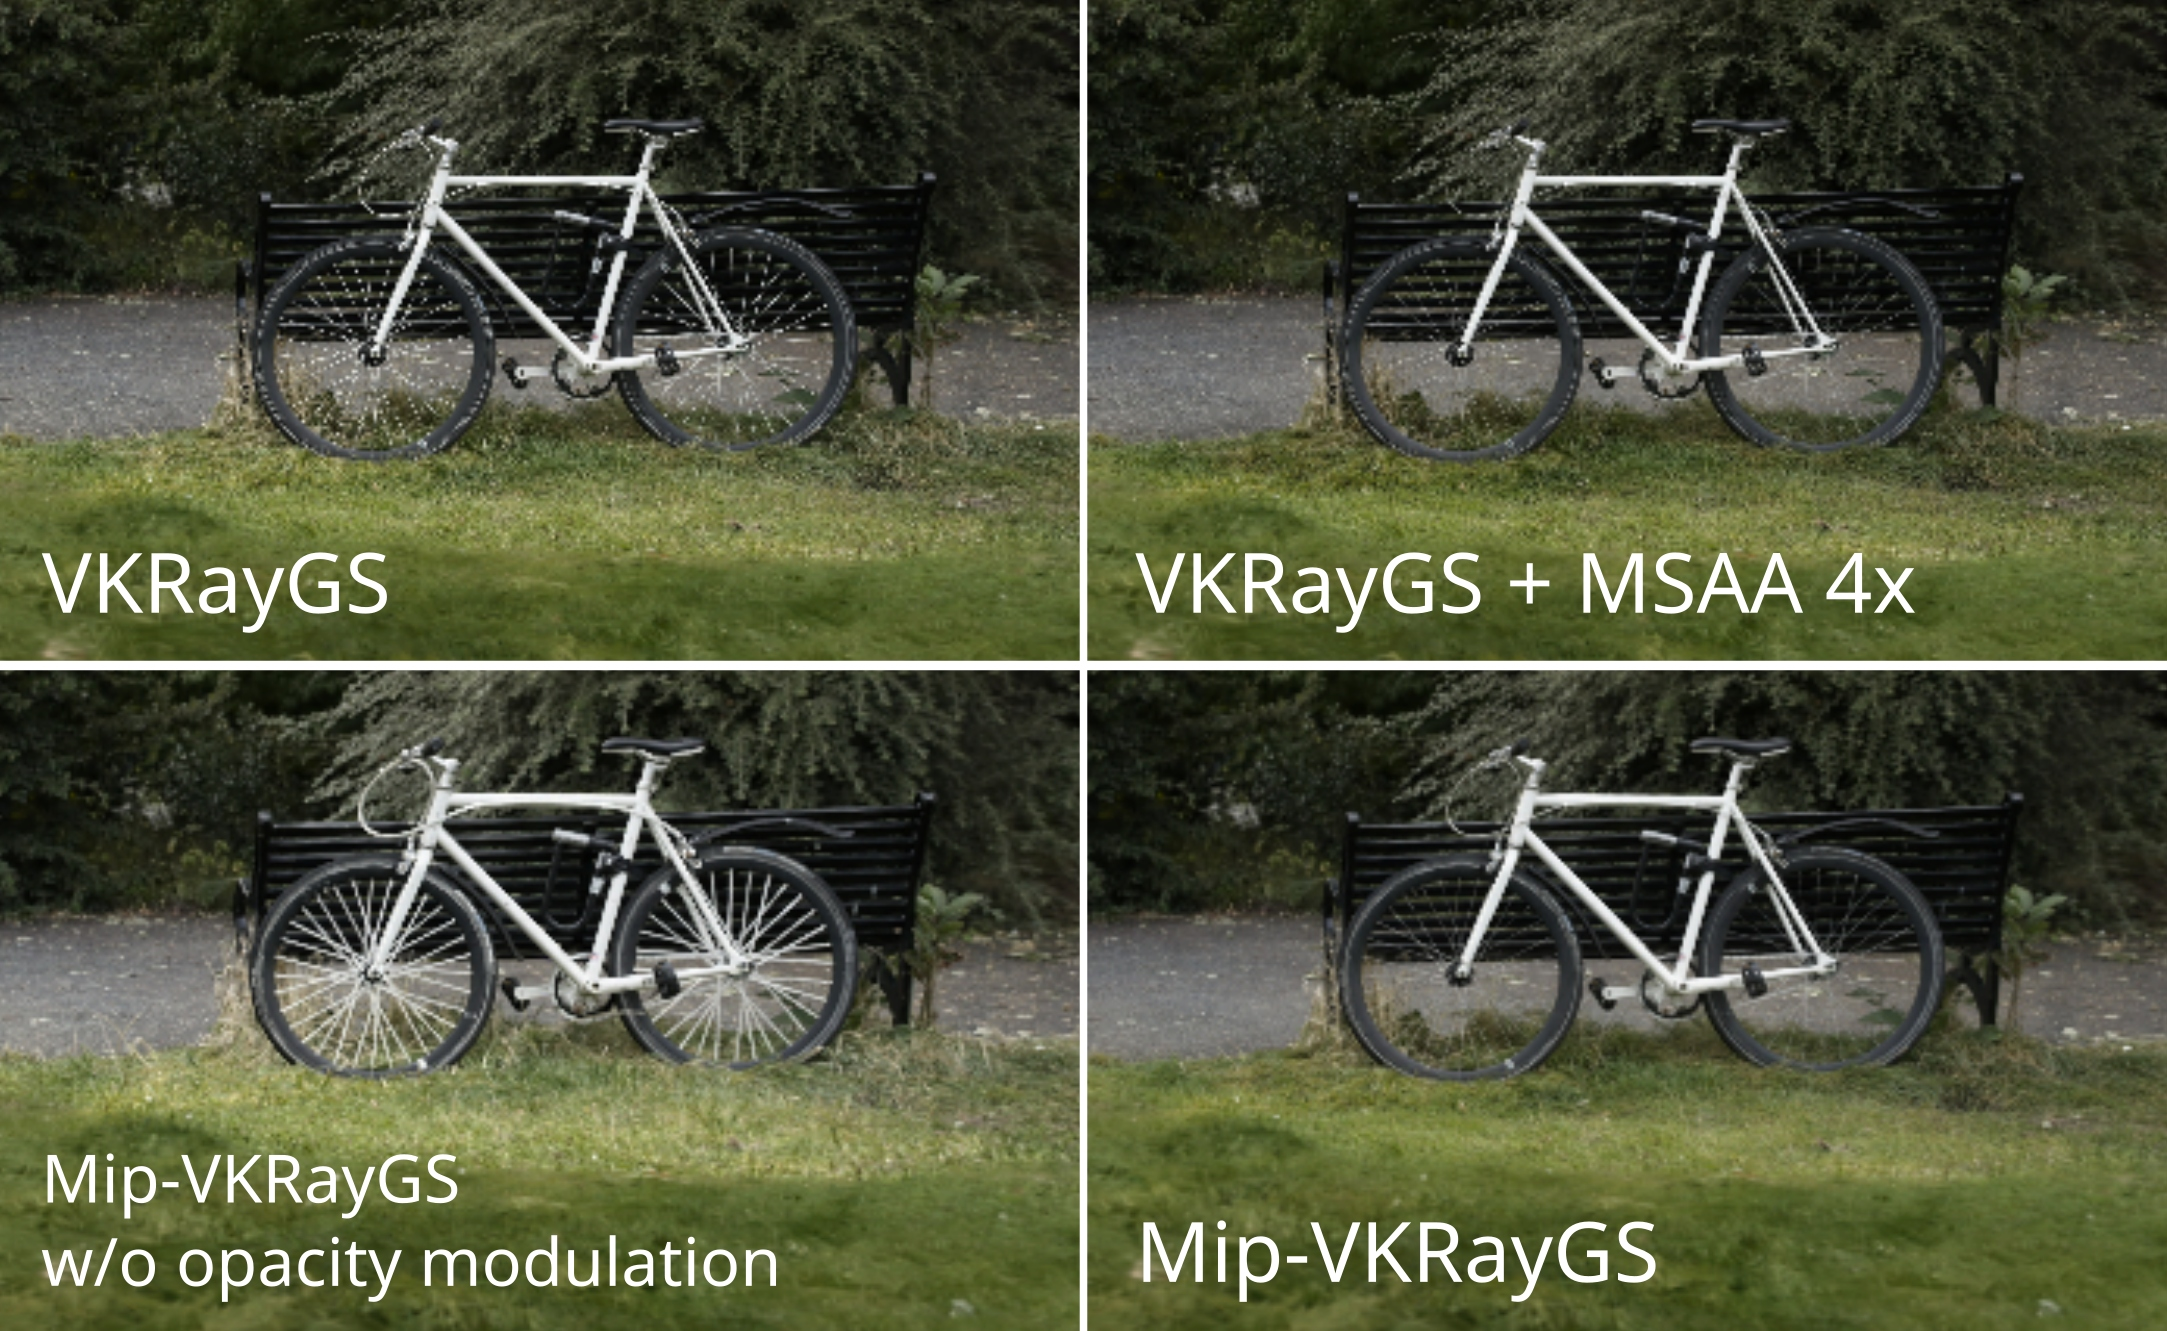
\includegraphics[width=\linewidth]{./figures/MIP.jpg}
    \caption{RayGS MIP 抗锯齿效果对比（论文图 4）}
\end{figure}

论文图 5 使用 room 场景展示相机靠近物体时的结果。上排 VKGS 出现尖刺状、不符合几何的 artifacts；下排 VKRayGS 更稳定。论文解释是 RayGS 的 opacity 计算在几何上更一致，不依赖普通 GS 的屏幕投影线性化近似。

\begin{figure}[H]
    \centering
    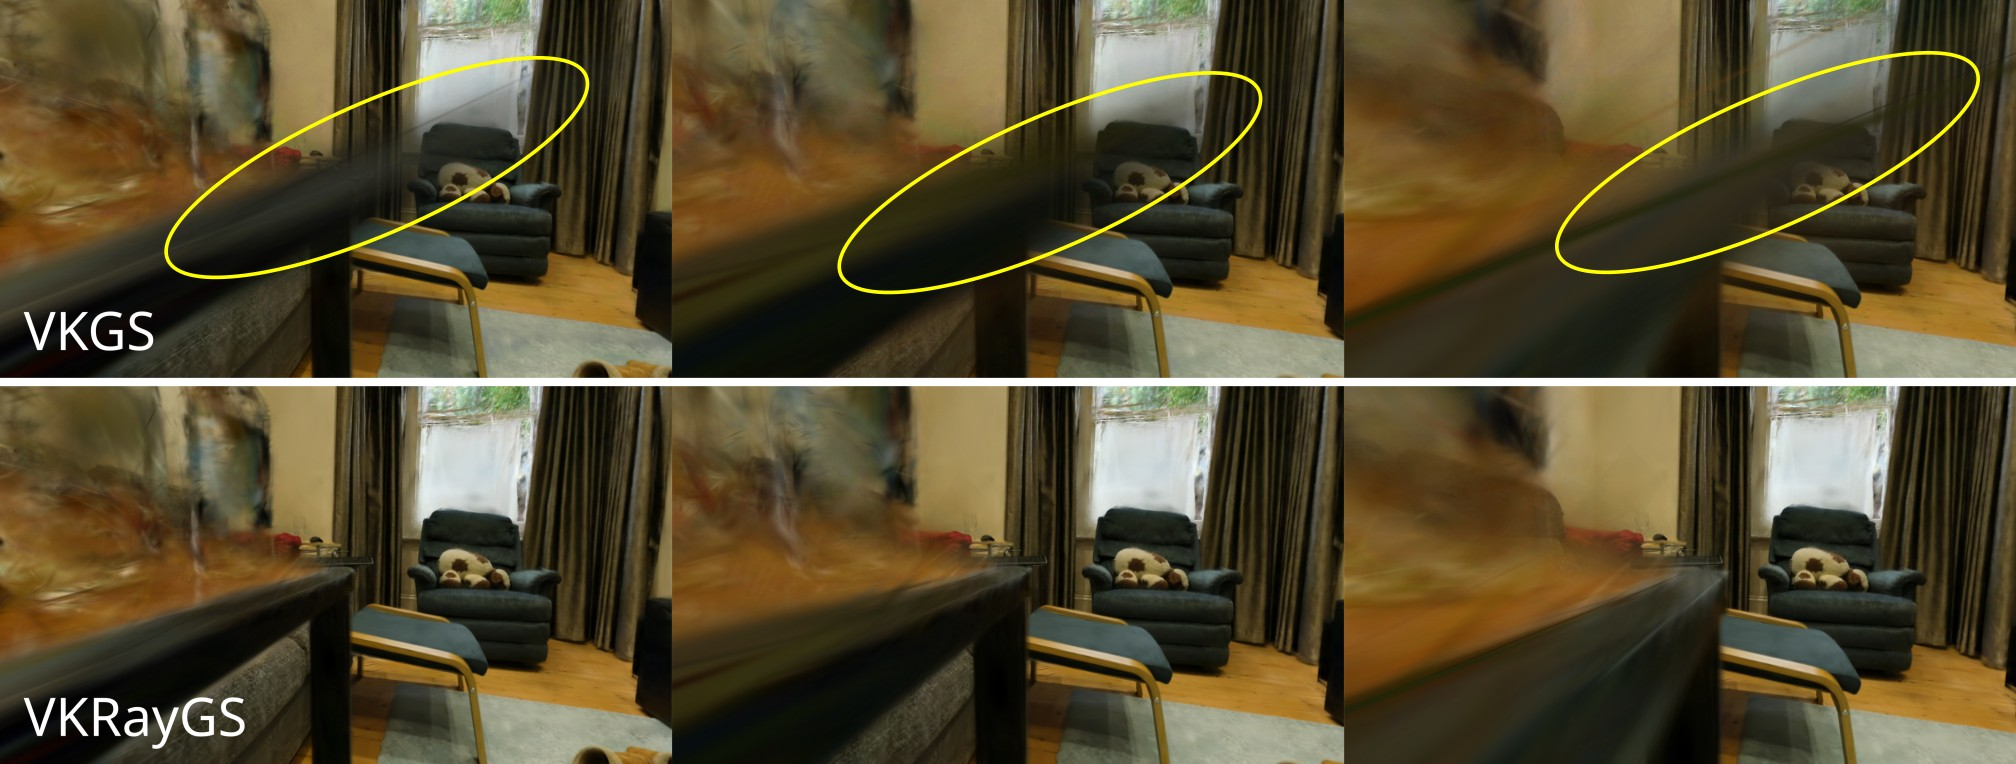
\includegraphics[width=\linewidth]{./figures/artifacts_highlighted.jpg}
    \caption{VKGS 与 VKRayGS 近距离伪影对比（论文图 5）}
\end{figure}



\subsection{论文实验的局限性}
论文实验仍有一些局限：

\begin{itemize}
    \item MIP 缺少大规模量化实验。论文主要通过图 4 展示 MIP 效果，没有在所有场景中报告开启 MIP 后的 PSNR、SSIM、LPIPS 和 FPS。
    \item 模型训练可能偏向 GOF。论文使用的模型来自竞争方法或由竞争方法代码训练，因此质量指标可能受到 renderer mismatch 影响。
    \item 硬件平台较单一。主实验在 RTX2080 上进行，虽然 Vulkan 理论上具有跨平台潜力，但论文没有充分展示不同 GPU/平台下的性能。
    \item 只加速测试时渲染，不加速训练。本文重点是 test-time renderer，训练阶段是否能用硬件光栅化加速仍是未来工作。
\end{itemize}



\section{本地复现实验与补充分析}
\subsection{复现目的}
在阅读论文实验部分的基础上，本组进一步使用作者公开的预训练 Gaussian 点云和 VKRayGS Viewer 进行了本地复现~\cite{inriags}。复现实验不重新训练模型，而是固定渲染模式、分辨率和相机视角，记录 FPS、帧时间、projection time、rendering time、visible ratio、显存占用与 GPU 功耗，并整理代表性截图用于比较质量、伪影和交互体验。

需要说明的是，本地复现得到的 FPS 与论文表格中的 FPS 不适合直接逐项对齐，差异主要来自测试设备、显卡性能、驱动和运行环境不同。因此，复现部分更侧重验证硬件光栅化 RayGS 的实时交互趋势，而不是完全复刻论文在 RTX2080 上的绝对帧率。



\subsection{VKRayGS 仓库结构与构建方式}
VKRayGS 官方代码~\footnotemark{} 基于 \texttt{vkgs} Viewer 开发~\cite{vkgs}，主要使用 Vulkan、GLFW、ImGui、GLM、Vulkan Memory Allocator 以及 Vulkan radix sort 等依赖。README 中给出的基础构建方式如下：

\footnotetext{\url{https://github.com/SLDRMK/vkraygs}}

\begin{lstlisting}[language=bash]
git submodule update --init --recursive
cmake . -B build
cmake --build build --config Release -j
./build/vkgs_viewer -i <ply_filepath>
\end{lstlisting}

复现指南中进一步补充了面向实验的脚本和参数。仓库中与实验复现关系最密切的文件如表~\ref{tab:repo_structure} 所示。

\begin{table}[H]
    \centering
    \caption{VKRayGS 仓库中与实验复现相关的主要文件}
    \label{tab:repo_structure}
    \setlength{\tabcolsep}{2pt}
    \renewcommand{\arraystretch}{1.2}
    \begin{tabular}{cc}
        \bottomrule[1.5pt]
        路径 & 作用 \\
        \midrule[0.5pt]
        examples/vkgs\_viewer.cc & Viewer 程序入口与命令行参数解析 \\
        src/vkgs/engine/engine.cc & 渲染模式切换、计时、主绘制逻辑、CSV 指标导出 \\
        src/shader/projection.comp & 传统 GS 投影路径 \\
        src/shader/raygs\_projection.comp & RayGS 投影路径 \\
        src/shader/splat.vert/.frag & GS 光栅化 shader \\
        src/shader/raygs\_splat.vert/.frag & RayGS 光栅化 shader \\
        all-in-one.sh & 单次实验入口，封装运行参数和输出整理 \\
        exp\_perf\_table1.sh & Table 1 风格性能复现实验 \\
        exp\_resolution\_sweep.sh & 分辨率扫描实验 \\
        exp\_gs\_vs\_raygs.sh & GS 与 RayGS 对比实验 \\
        exp\_mip\_sweep.sh & MIP / MSAA 抗锯齿实验 \\
        exp\_nearfield\_manual.sh & 近景手动观察、截图或录屏实验 \\
        run\_all\_experiments.sh & 自动化实验总入口 \\
        build\_tables.py & 汇总 Viewer 与 GPU CSV，生成总表 \\
        experiment-results/ & 实验输出目录 \\
        \toprule[1.5pt]
    \end{tabular}
\end{table}



\subsection{数据来源与相机控制}
实验不重新训练模型，而是使用 3D Gaussian Splatting 官方预训练模型~\cite{inriags}。复现指南中假设的数据目录如下：

\begin{lstlisting}
ComputerGraphics/
    models/
        bicycle/
            cameras.json
            cfg_args
            point_cloud/iteration_30000/point_cloud.ply
        garden/
        room/
        bonsai/
        truck/
    vkraygs/
\end{lstlisting}

\texttt{point\_cloud.ply} 是 Viewer 实际加载的 Gaussian 模型，\texttt{cameras.json} 保存训练或数据集导出的相机参数。实验脚本支持从 \texttt{cameras.json} 中读取相机位置、朝向、上方向、焦距和图像尺寸，覆盖默认 Viewer 视角。

除近景手动实验外，批处理脚本默认使用：

\begin{lstlisting}[language=bash]
CAMERA_SAMPLE_COUNT=10
CAMERA_SAMPLE_SEED=20250618
\end{lstlisting}

同一个场景、同一个随机种子和同一个抽样数量会稳定得到同一组 camera id。bicycle 的 $1920\times1080$ RayGS 基准配置重复运行 3 组，共 30 次，因此既可以观察视角差异，也可以检查重跑稳定性。



\subsection{渲染模式、实验参数与记录方式}
复现指南中列出了当前 Viewer 支持的主要渲染模式：

\begin{itemize}
    \item \textbf{GS / VKGS}：使用 \texttt{projection.comp}、\texttt{splat.vert} 和 \texttt{splat.frag}；
    \item \textbf{RayGS / VKRayGS}：使用 \texttt{raygs\_projection.comp}、使用 \texttt{raygs\_splat.vert} 和使用 \texttt{raygs\_splat.frag}，是当前默认模式；
    \item \textbf{Geometry Shader GS}：通过 geometry shader 扩展 splat；
    \item \textbf{Mip-GS / Mip-RayGS}：通过设置 \texttt{mip\_bias > 0} 且开启 \texttt{mip\_modulation} 实现；
    \item \textbf{MSAA}：通过 \texttt{2x} 或 \texttt{4x} 多重采样叠加在当前渲染模式上。
\end{itemize}

一次典型自动化实验命令如下：

\begin{lstlisting}[language=bash]
./run.sh \
    --input /path/to/model.ply \
    --width 1920 \
    --height 1080 \
    --display-mode windowed \
    --vsync off \
    --msaa off \
    --depth f32 \
    --draw-method triangles \
    --model-type raygs \
    --mip-bias 0.0 \
    --mip-modulation on \
    --log-p-min -4.0 \
    --axis off \
    --grid off \
    --metrics-csv /tmp/viewer_metrics.csv \
    --warmup-sec 5 \
    --capture-sec 10 \
    --auto-exit on
\end{lstlisting}

这些参数保证实验时关闭垂直同步，禁用辅助网格和坐标轴，并在预热后自动采集一段时间的性能数据。Viewer 会导出逐帧 CSV，脚本同时调用 \texttt{nvidia-smi} 采集 GPU 指标，再通过 \texttt{build\_tables.py} 汇总为 \texttt{run\_summary.csv}。

复现指南强调性能采集与视觉材料采集应分开进行。截图和录屏会占用 GPU 编码器、显存带宽和显示管线，因此截图/录屏时的 FPS 不应作为正式性能数据。



\subsection{实验结果目录}
\texttt{experiment-results/} 中保存四类结果：

\begin{itemize}
    \item \texttt{gpu/}：每次运行的 \texttt{nvidia-smi} 采样 CSV 及摘要；
    \item \texttt{metrics/}：Viewer 导出的逐帧指标 CSV 及摘要；
    \item \texttt{screenshots/}：典型视角下的主观比较截图；
    \item \texttt{tables/run\_summary.csv}：汇总表。
\end{itemize}

本次读取到的 \texttt{run\_summary.csv} 共包含 160 条运行记录。字段可以分为四类：

\begin{itemize}
    \item 基本配置：\texttt{scene}、\texttt{resolution}、\texttt{model\_type}、\texttt{draw\_method}、\texttt{msaa}、\texttt{vsync}、\texttt{mip\_bias}、\texttt{mip\_modulation} 和 \texttt{log\_p\_min}；
    \item Viewer 性能：\texttt{fps\_avg}、\texttt{fps\_max}、\texttt{frame\_time\_avg\_ms}、\texttt{frame\_e2e\_avg\_ms} 以及 \texttt{projection\_avg\_ms} 和 \texttt{rendering\_avg\_ms}；
    \item 场景负载：\texttt{visible\_ratio\_avg} 和 \texttt{total\_splats}；
    \item GPU 指标包含：\texttt{gpu\_util\_avg}、\texttt{gpu\_util\_max}、\texttt{vram\_used\_max\_mib}、\texttt{power\_avg\_w}、\texttt{vram\_used\_avg\_mib}、\texttt{power\_max\_w}。
\end{itemize}



\subsection{本地结果一：不同场景整体性能}

\begin{table}[H]
    \centering
    \caption{本地复现实验设置}
    \setlength{\tabcolsep}{2pt}
    \renewcommand{\arraystretch}{1.5}
    \resizebox{\textwidth}{!}{
        \begin{tabular}{cc}
            \bottomrule[1.5pt]
            \textbf{项目} & \textbf{设置} \\
            \midrule[0.5pt]
            数据来源 & 作者公开 3D Gaussian Splatting 预训练模型 \texttt{point\_cloud.ply} \\
            主要场景 & bicycle、garden、room、bonsai、truck \\
            默认渲染配置 & RayGS；Triangles 绘制路径；Vsync 关闭；Depth F32；MIP modulation 开启；\texttt{log\_p\_min=-4} \\
            视角来源 & 从 \texttt{cameras.json} 固定随机种子抽样；近景实验采用手动 dolly far/mid/near \\
            记录指标 & FPS、frame time、projection/rendering time、visible ratio、GPU/VRAM/power \\
            截图对比 & GS、RayGS、Mip-RayGS、MSAA 4x；bicycle 近景 far/mid/near；truck 代表视角 \\
            \toprule[1.5pt]
        \end{tabular}
    }
\end{table}

\begin{table}[H]
    \centering
    \caption{本地复现实验：整体性能概览}
    \label{tab:local_overall_perf}
    \setlength{\tabcolsep}{4pt}
    \renewcommand{\arraystretch}{1.2}
    \begin{tabular}{cccccc}
        \bottomrule[1.5pt]
        \textbf{场景} & \textbf{样本数} & \textbf{平均 FPS} & \textbf{FPS 最小/最大} & \textbf{平均帧时间 ms} & \textbf{Gaussian 数 M} \\
        \midrule[0.5pt]
        bicycle & 30 & 506.52 & 455.50 / 594.25 & 1.991 & 6.13 \\
        bonsai & 10 & 878.20 & 777.93 / 1002.93 & 1.147 & 1.24 \\
        garden & 10 & 398.88 & 350.63 / 443.97 & 2.518 & 5.83 \\
        room & 10 & 737.50 & 550.95 / 963.40 & 1.395 & 1.59 \\
        truck & 10 & 526.18 & 444.90 / 577.89 & 1.918 & 2.54 \\
        \toprule[1.5pt]
    \end{tabular}
\end{table}

\begin{table}[H]
    \centering
    \caption{本地复现实验：阶段耗时与可见比例}
    \label{tab:local_stage_perf}
    \setlength{\tabcolsep}{30pt}
    \renewcommand{\arraystretch}{1.2}
    \begin{tabular}{cccc}
        \bottomrule[1.5pt]
        \textbf{场景} & \textbf{投影 ms} & \textbf{渲染 ms} & \textbf{可见比例 \%} \\
        \midrule[0.5pt]
        bicycle & 0.717 & 0.779 & 25.48 \\
        bonsai & 0.192 & 0.750 & 33.32 \\
        garden & 1.050 & 0.904 & 35.65 \\
        room & 0.194 & 0.976 & 26.91 \\
        truck & 0.468 & 1.113 & 41.93 \\
        \toprule[1.5pt]
    \end{tabular}
\end{table}

\begin{figure}[H]
    \centering
    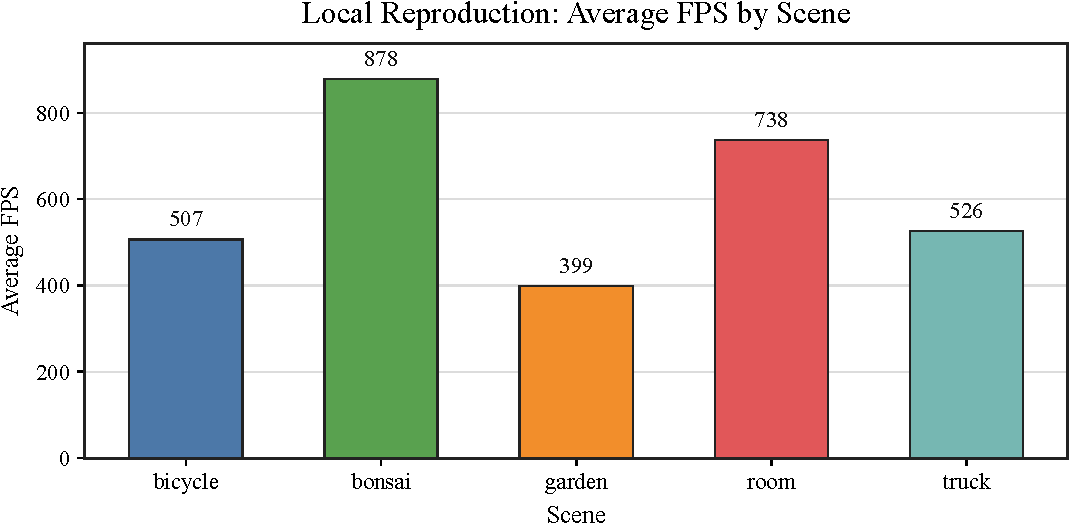
\includegraphics[width=\linewidth]{./figures/average_fps_by_scene_beautified.pdf}
    \caption{本地复现实验各场景平均 FPS}
\end{figure}

从整体结果看，RayGS 在 $1920\times1080$ 下全部测试场景均达到实时交互帧率，平均 FPS 从 garden 的约 399 FPS 到 bonsai 的约 878 FPS 不等。bicycle 和 garden 的 Gaussian 数分别约为 6.13M 和 5.83M，projection 耗时明显高于 room、bonsai；truck 虽然总点数约 2.54M，但可见比例约 41.93\%，rendering 阶段耗时较高。可见，性能瓶颈不能只用模型总点数解释，还需要结合当前视角下参与光栅化的 splat 数量、像素覆盖和遮挡关系。

bicycle 在 30 次 $1920\times1080$ RayGS 基准运行中的平均 FPS 为 506.52，单视角平均 FPS 约在 455.50 到 594.25 之间波动。当前景细节、车轮辐条、植被和遮挡层次较多时，projection 与 rendering 时间都会上升；视角更开阔或可见 splat 较少时帧率更高。这说明同一模型在不同观察方向下负载差异明显，课程报告中只给单个 FPS 容易低估视角因素。



\subsection{本地结果二：分辨率、MSAA 与 MIP 影响}

\begin{table}[H]
    \centering
    \caption{bicycle：分辨率、MSAA 与 MIP 影响}
    \label{tab:local_resolution_msaa_mip}
    \setlength{\tabcolsep}{6pt}
    \renewcommand{\arraystretch}{1.2}
    \begin{tabular}{cccccc}
        \bottomrule[1.5pt]
        \textbf{设置} & \textbf{样本数} & \textbf{平均 FPS} & \textbf{帧时间 ms} & \textbf{投影 ms} & \textbf{渲染 ms} \\
        \midrule[0.5pt]
        720p / 1x / MIP0 & 10 & 621.37 & 1.626 & 0.714 & 0.437 \\
        1080p / 1x / MIP0 & 30 & 506.52 & 1.991 & 0.717 & 0.779 \\
        1080p / 1x / MIP0.05 & 10 & 497.56 & 2.027 & 0.723 & 0.811 \\
        1080p / 1x / MIP0.10 & 10 & 495.22 & 2.037 & 0.722 & 0.822 \\
        1080p / 1x / MIP0.20 & 10 & 491.49 & 2.053 & 0.725 & 0.837 \\
        1080p / 2x / MIP0 & 10 & 409.08 & 2.470 & 0.728 & 1.281 \\
        1080p / 4x / MIP0 & 10 & 323.75 & 3.128 & 0.727 & 1.936 \\
        2490$\times$1376 / 1x / MIP0 & 20 & 424.98 & 2.374 & 0.723 & 1.143 \\
        \toprule[1.5pt]
    \end{tabular}
\end{table}

\begin{figure}[H]
    \centering
    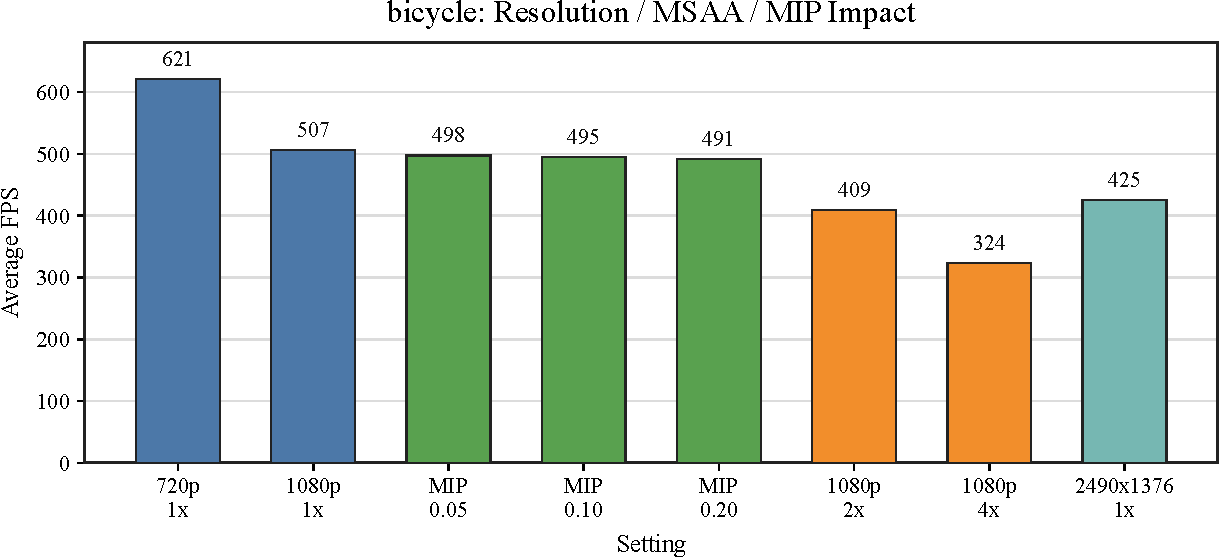
\includegraphics[width=\linewidth]{./figures/bicycle_resolution_msaa_mip_impact_beautified.pdf}
    \caption{bicycle 场景中分辨率、MSAA 与 MIP 对 FPS 的影响}
\end{figure}

bicycle 分辨率扫描显示，$1280\times720$ 下平均约 621.37 FPS，$1920\times1080$ 基准约 506.52 FPS，而 $2490\times1376$ 下约 424.98 FPS。随着像素数增加，projection 耗时基本维持在 0.72 ms 左右，主要增长来自 rendering 阶段，符合硬件光栅化路径中像素填充和片元处理成本随分辨率升高而增加的预期。

MSAA 对性能的影响更直接：$1920\times1080$ 下 2x MSAA 平均约 409.08 FPS，4x MSAA 下降到约 323.75 FPS；对应 rendering 平均耗时从基准约 0.779 ms 上升到 1.281 ms 和 1.936 ms，而 projection 时间几乎不变。MIP bias 从 0 增大到 0.05、0.10、0.20 后，FPS 略有下降但幅度不大；从截图观察，MIP 更适合作为远处细节稳定性调节项，而不是主要性能优化项。



\subsection{本地结果三：GS 与 RayGS 对比}

\begin{table}[H]
    \centering
    \caption{truck 场景：GS 与 RayGS 对比}
    \label{tab:local_gs_raygs_truck}
    \setlength{\tabcolsep}{6pt}
    \renewcommand{\arraystretch}{1.2}
    \begin{tabular}{ccccccc}
        \bottomrule[1.5pt]
        \textbf{模型} & \textbf{样本数} & \textbf{平均 FPS} & \textbf{帧时间 ms} & \textbf{投影 ms} & \textbf{渲染 ms} & \textbf{平均功耗 W} \\
        \midrule[0.5pt]
        GS & 10 & 529.45 & 1.909 & 0.429 & 1.141 & 211.2 \\
        RayGS & 10 & 526.18 & 1.918 & 0.468 & 1.113 & 231.2 \\
        \toprule[1.5pt]
    \end{tabular}
\end{table}

在 truck 场景的同一批 10 个视角上，GS 与 RayGS 的平均 FPS 分别约为 529.45 和 526.18，整体帧率非常接近。RayGS 的 projection 阶段略高于 GS，但 rendering 阶段略低，因此总帧时间差距较小。结合论文结论可以理解为：RayGS 的价值不一定体现为相对 GS 的绝对 FPS 提升，而是以接近普通 GS 的实时性能换取更稳定的局部几何、遮挡边界和近景观察质量。



\subsection{代表性截图与主观分析}
截图结果集中在 \texttt{experiment-results/screenshots}，包括 bicycle 的 cam0、cam6，bicycle 近景 far/mid/near，以及 truck 的 cam0、cam6。整体上，GS 与 RayGS 在远景和中等距离下的颜色、结构和遮挡关系基本一致，说明 RayGS 没有破坏 3DGS 的全局主观质量；差异主要出现在物体边缘、细杆状结构、重复纹理以及近景放大区域。

bicycle 场景的车轮、辐条、车架和背景植被属于高频区域。普通 GS 在局部边缘容易出现轻微膨胀、半透明重叠和闪烁感；RayGS 的边缘收敛更自然，近景下 Gaussian 椭圆片带来的 billboard 感相对减弱。Mip-RayGS 在远处细节上更平滑，可以压制部分噪声，但也会让极细结构略显模糊。MSAA 4x 对高对比度轮廓有帮助，但无法根本解决由 Gaussian 表达本身引入的透明叠加和错误深度排序问题。

近景 far/mid/near 截图表明，随着相机靠近模型，传统 GS 的局部椭圆片形状更容易被看见，边界处会出现浮动、孔洞或局部过度模糊。RayGS 在近景下的交互观感更稳定，尤其是前景物体与背景交界处的形状更连贯；但在极端靠近或明显离开训练视角时，仍会保留 3DGS 模型本身的重建缺陷，例如背景区域破碎、反射或透明区域不稳定等。

\begin{figure}[H]
    \centering
    \begin{subfigure}{0.45\linewidth}
        \centering
        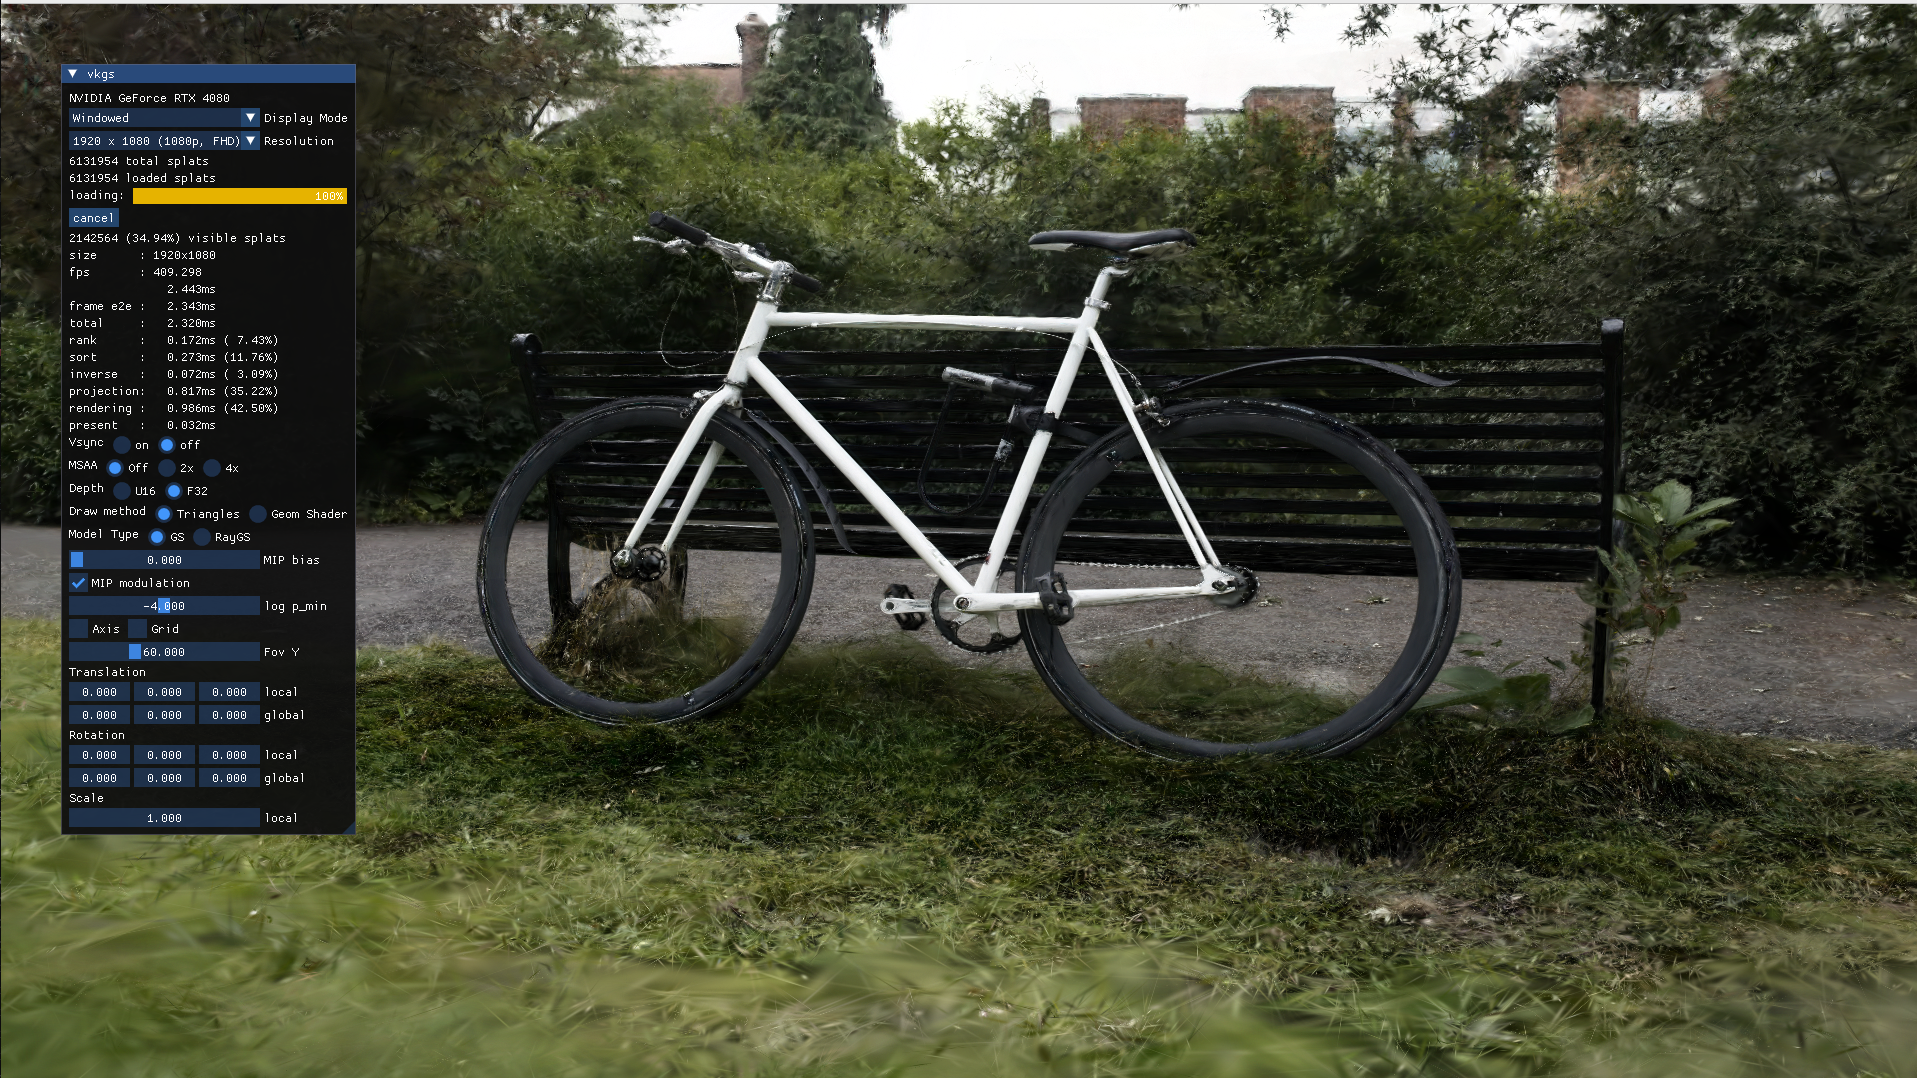
\includegraphics[width=\linewidth]{./figures/bicycle_cam0_gs.png}
        \caption{GS}
    \end{subfigure}
    \hfill
    \begin{subfigure}{0.45\linewidth}
        \centering
        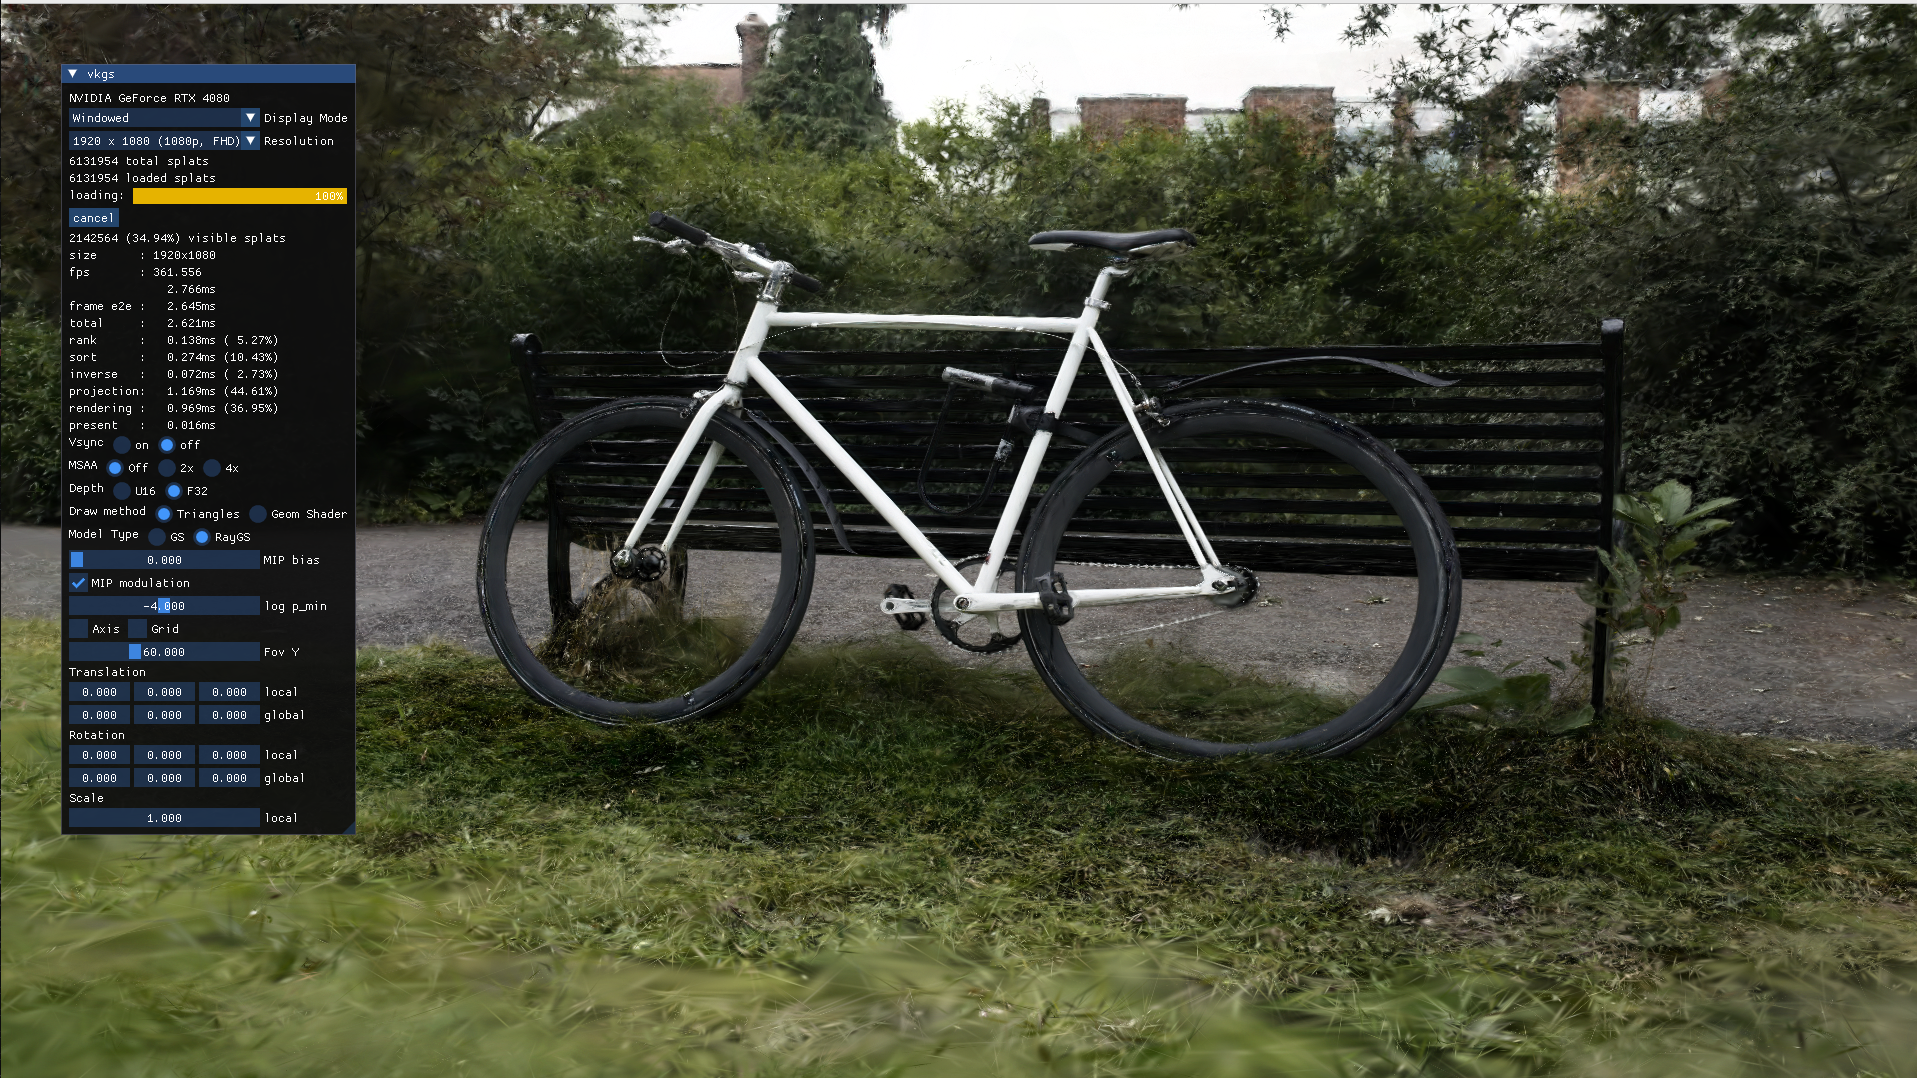
\includegraphics[width=\linewidth]{./figures/bicycle_cam0_raygs.png}
        \caption{RayGS}
    \end{subfigure}

    \vspace{0.6em}

    \begin{subfigure}{0.45\linewidth}
        \centering
        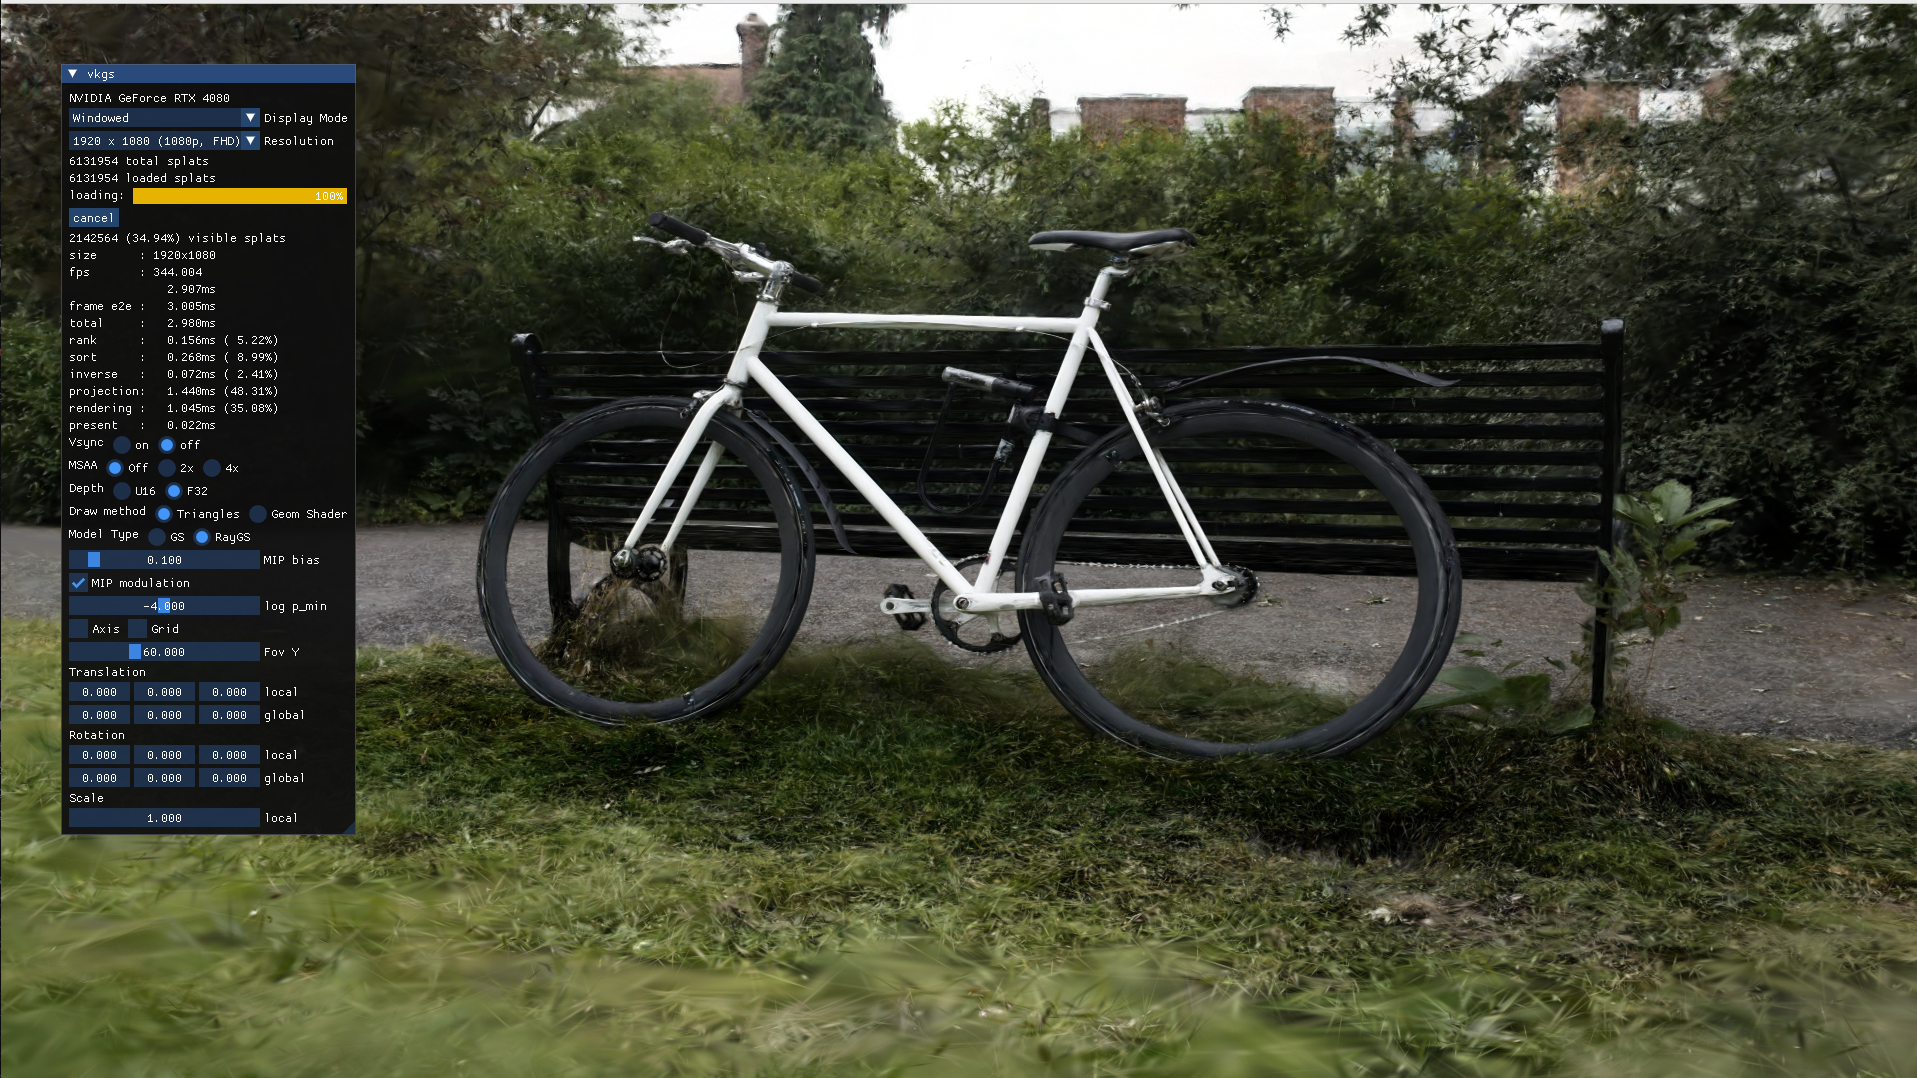
\includegraphics[width=\linewidth]{./figures/bicycle_cam0_mipraygs.png}
        \caption{MIP-RayGS}
    \end{subfigure}
    \hfill
    \begin{subfigure}{0.45\linewidth}
        \centering
        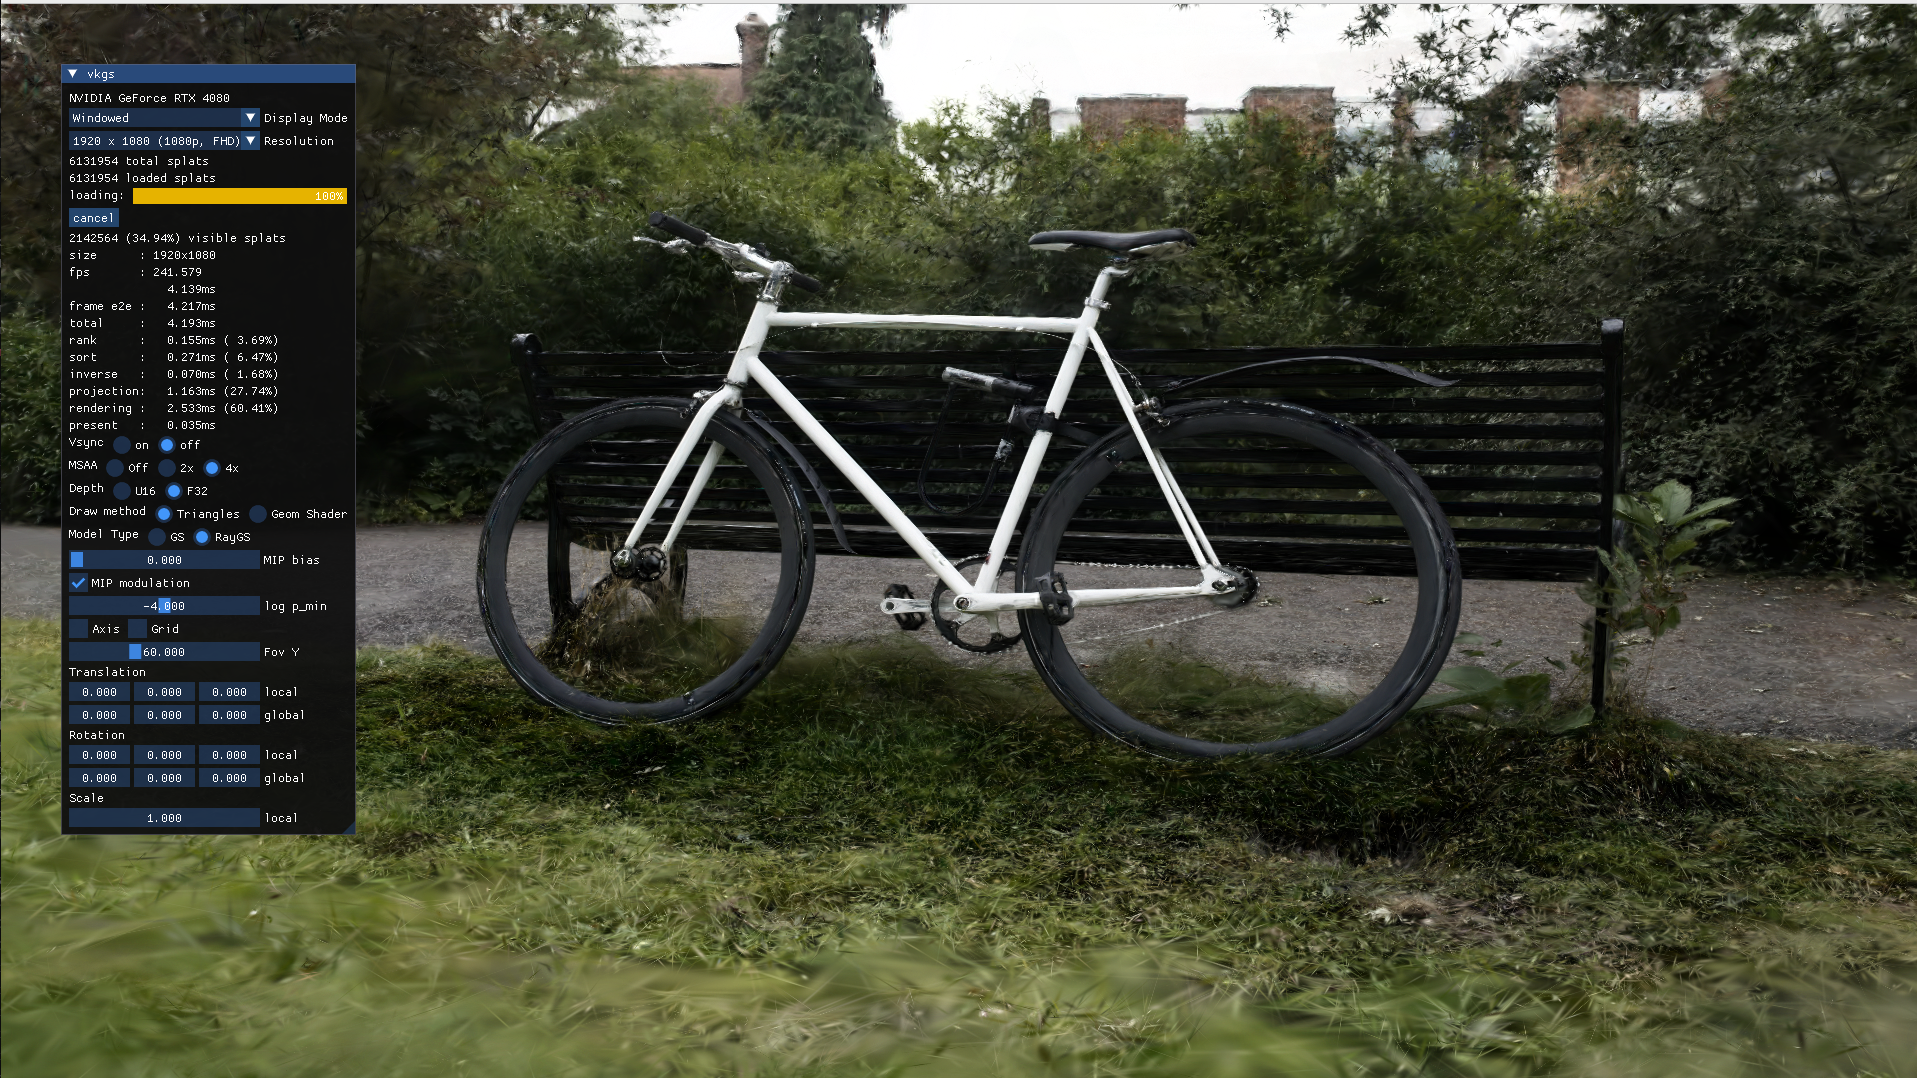
\includegraphics[width=\linewidth]{./figures/bicycle_cam0_msaa4x.png}
        \caption{MSAA 4x}
    \end{subfigure}
    \caption{bicycle cam0：GS、RayGS、MIP-RayGS 与 MSAA 4x 对比}
\end{figure}

\begin{figure}[H]
    \centering
    \begin{subfigure}{0.45\linewidth}
        \centering
        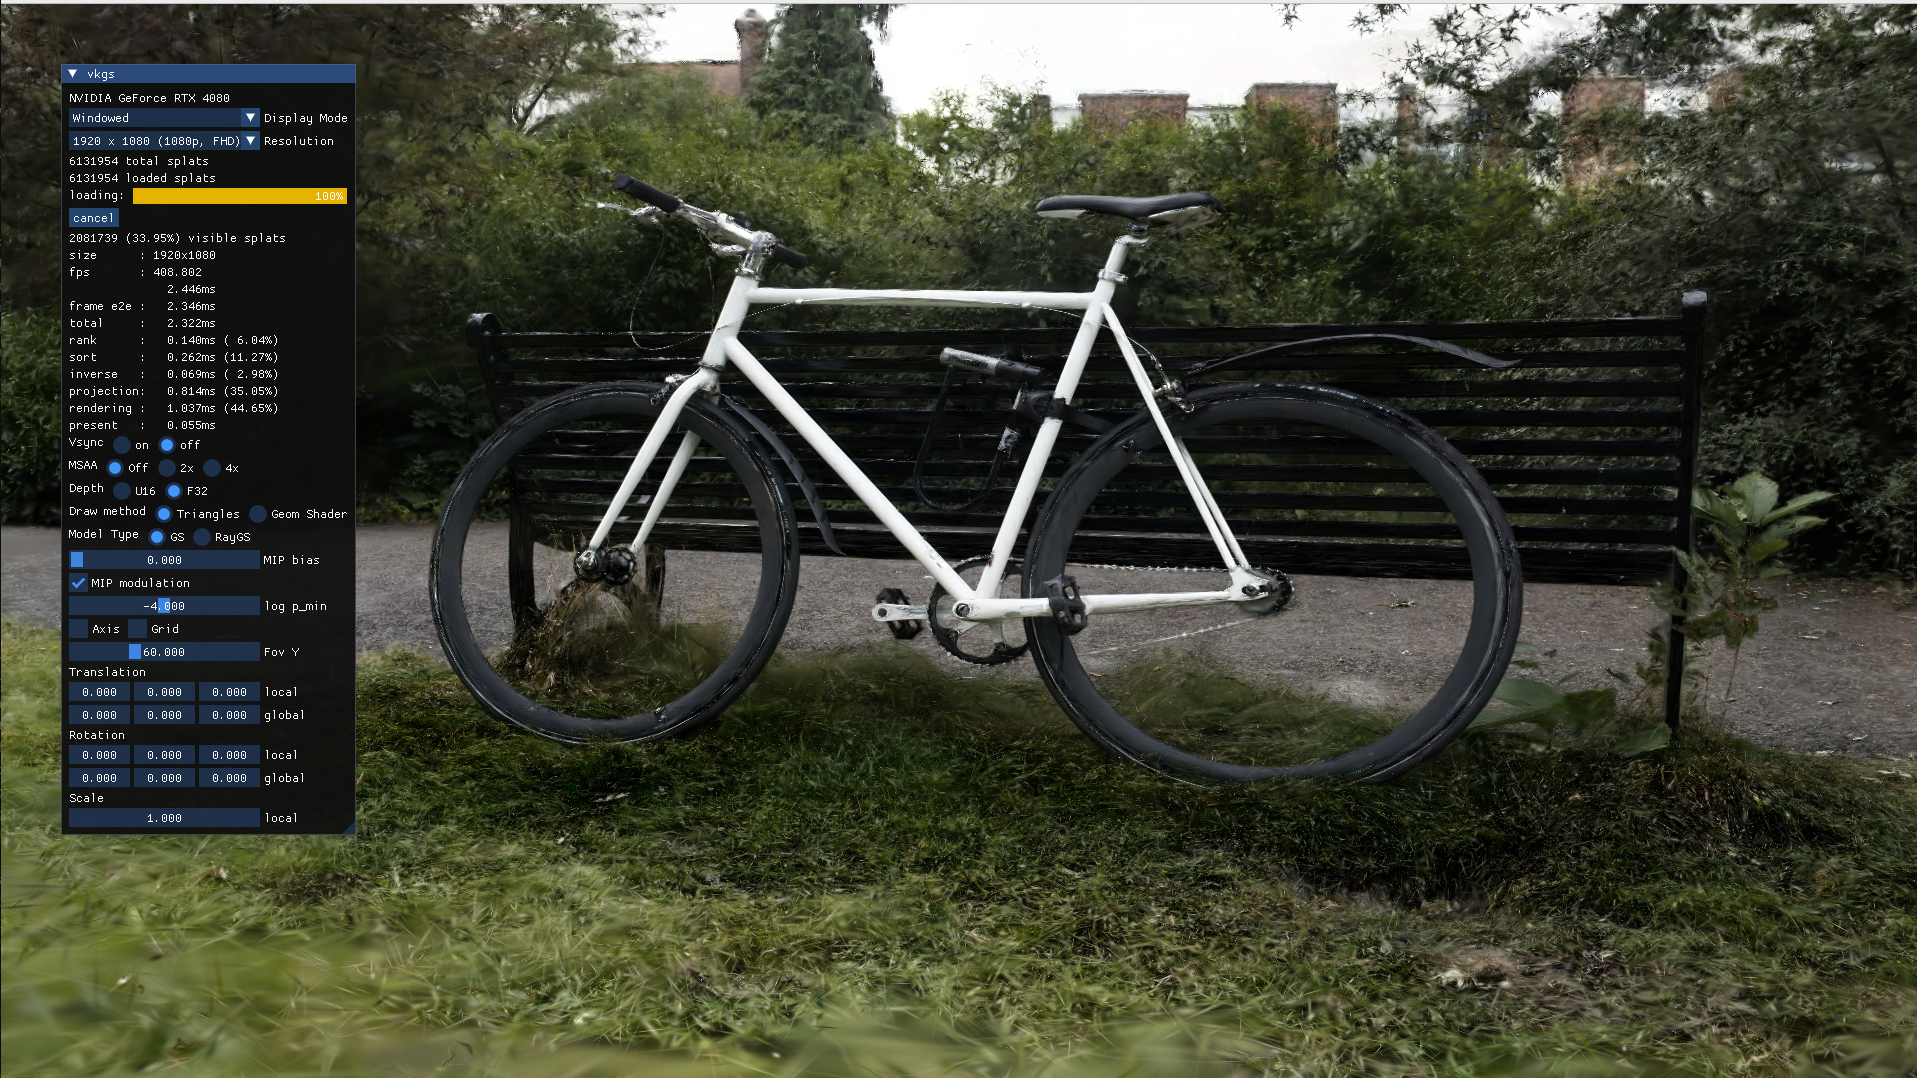
\includegraphics[width=\linewidth]{./figures/bicycle_near_gs_near.png}
        \caption{GS}
    \end{subfigure}
    \hfill
    \begin{subfigure}{0.45\linewidth}
        \centering
        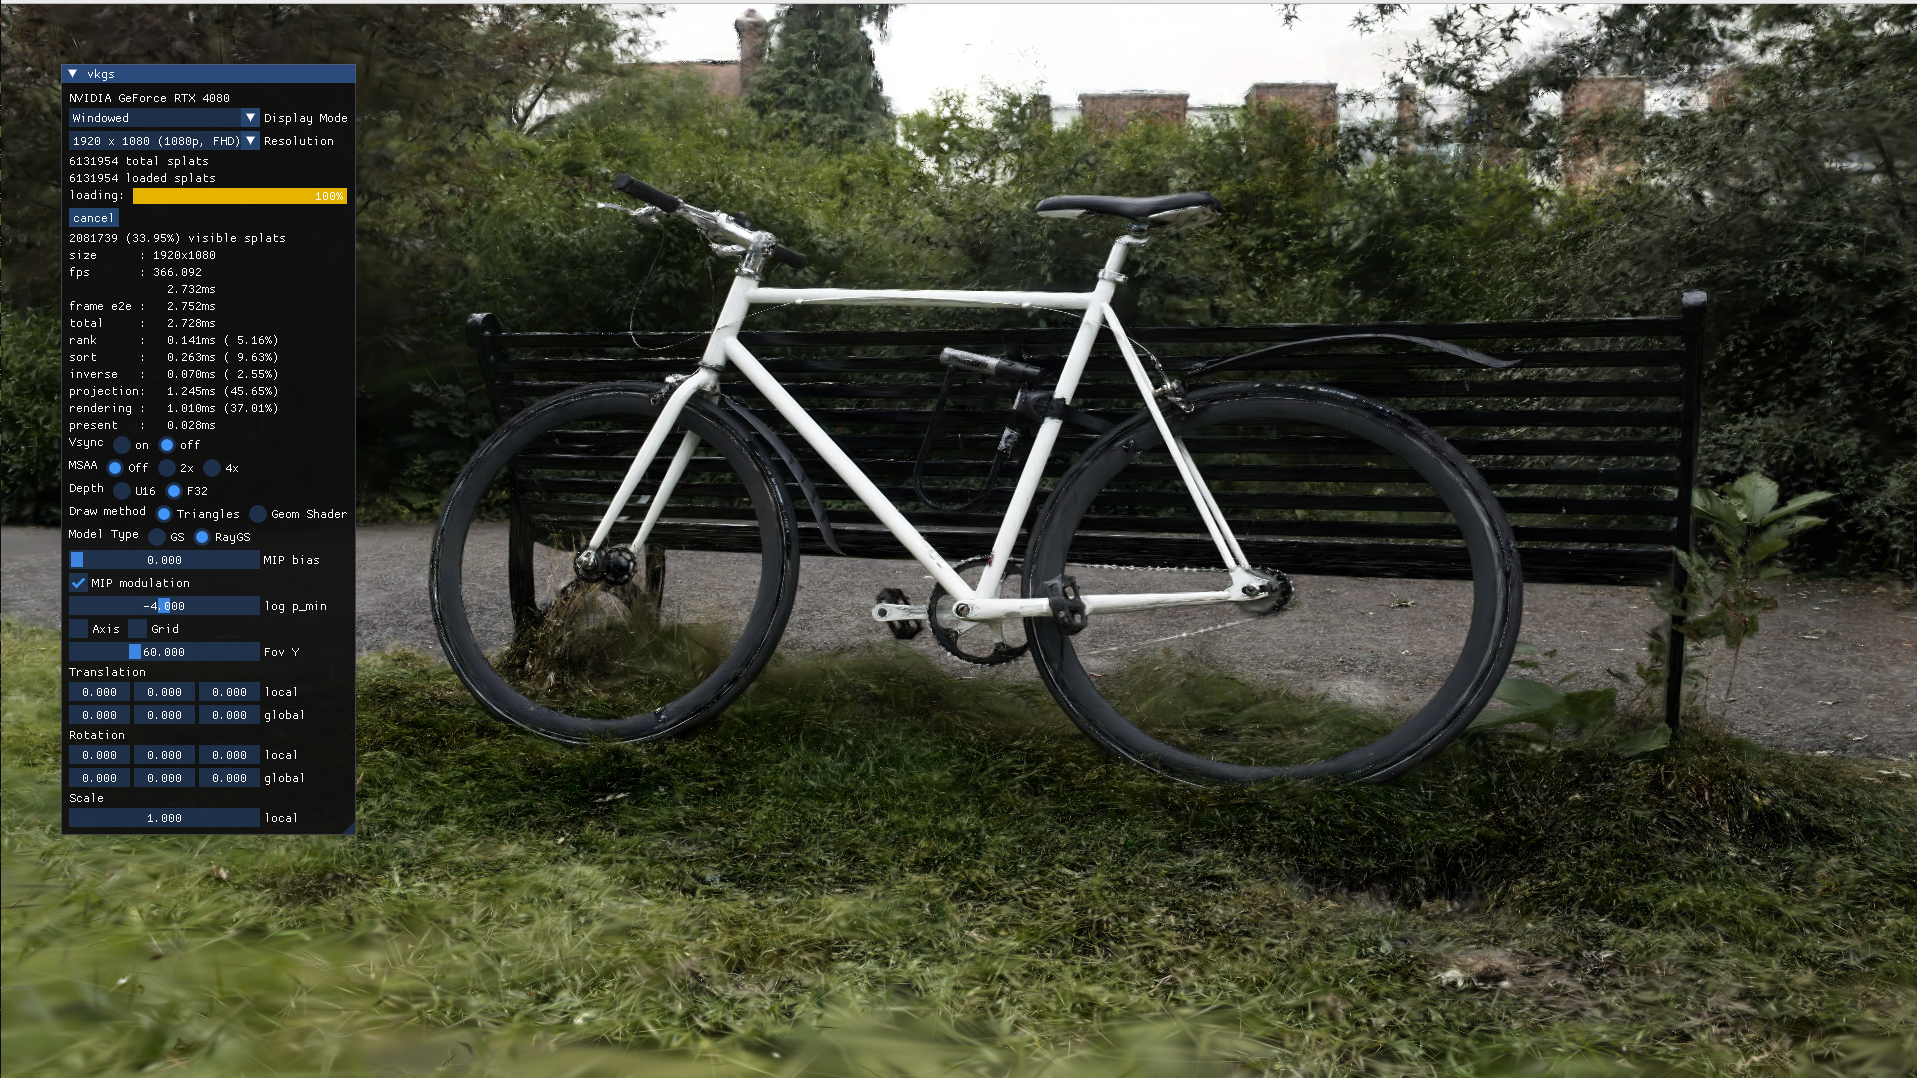
\includegraphics[width=\linewidth]{./figures/bicycle_near_raygs_near.png}
        \caption{RayGS}
    \end{subfigure}
    \caption{bicycle 近景：GS 与 RayGS 对比}
\end{figure}

\begin{figure}[H]
    \centering
    \begin{subfigure}{0.45\linewidth}
        \centering
        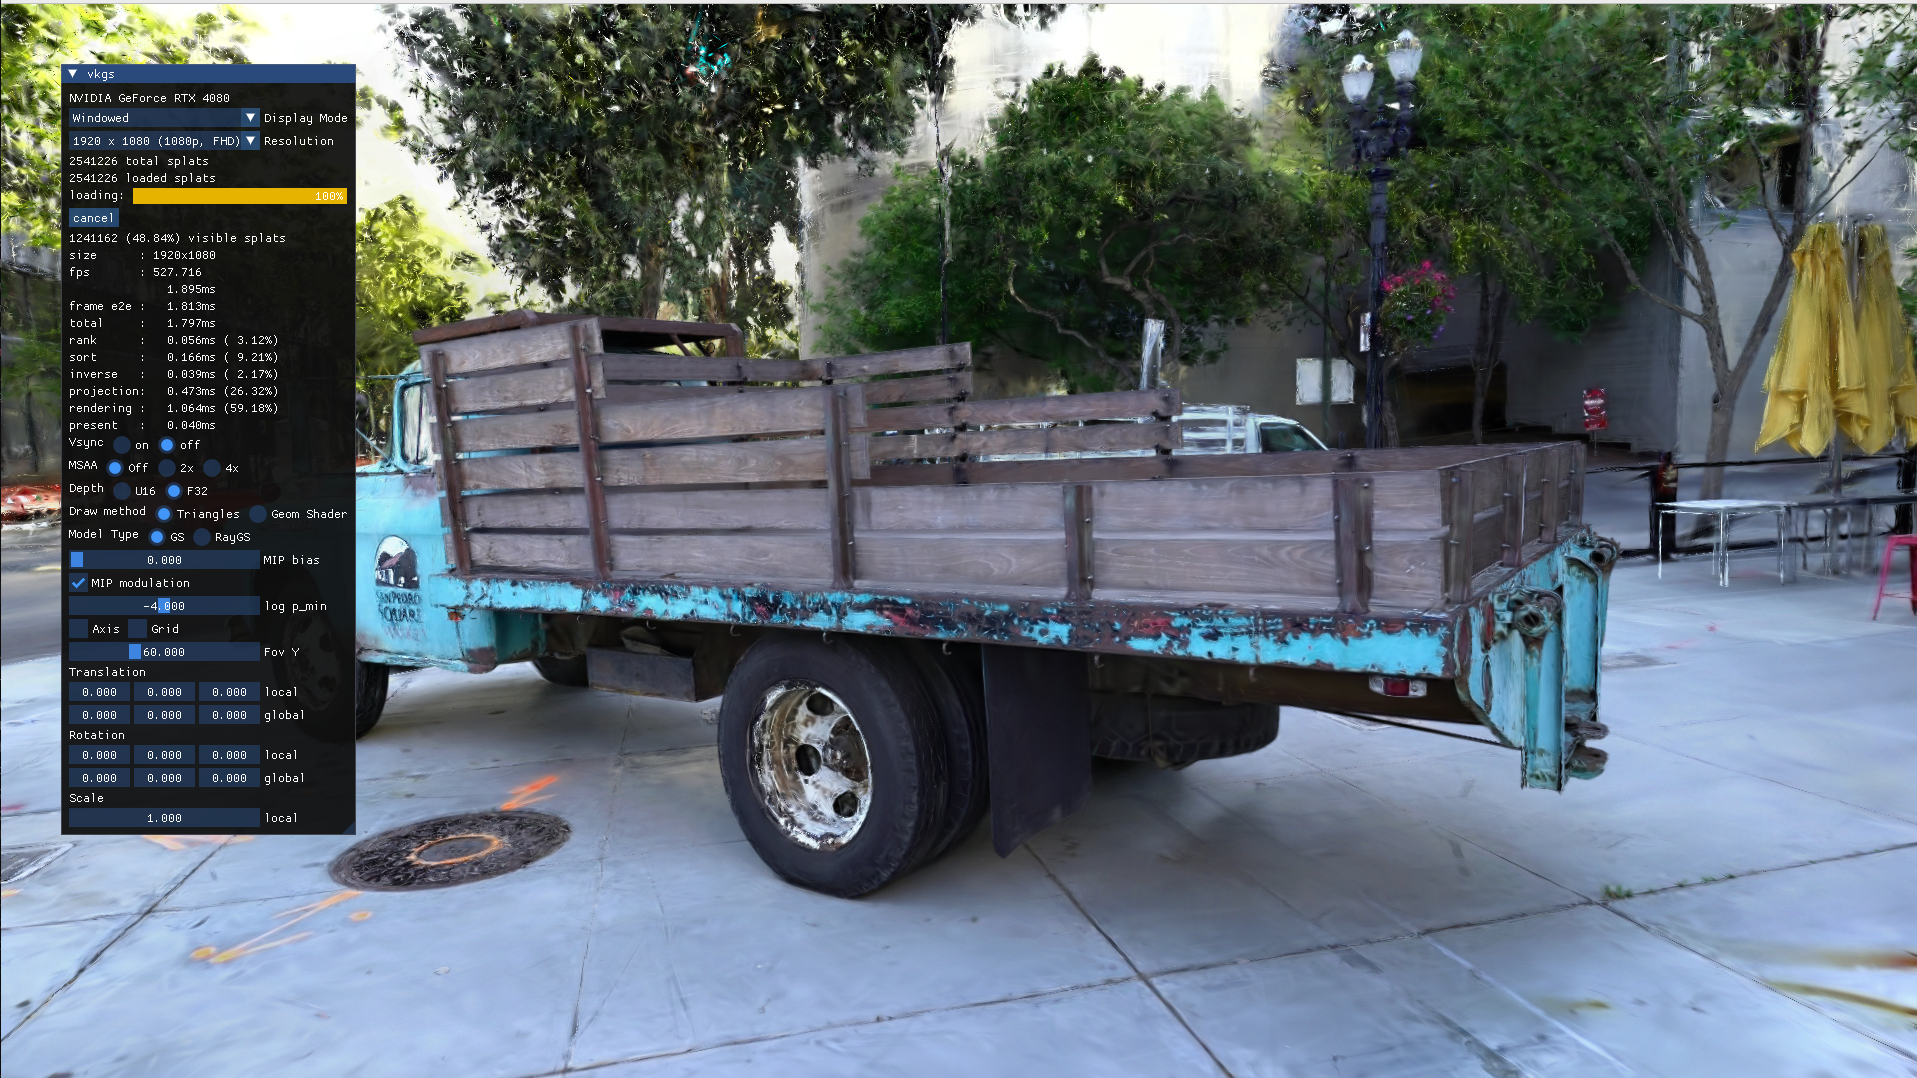
\includegraphics[width=\linewidth]{./figures/truck_cam0_gs.png}
        \caption{\texttt{truck\_cam0\_gs.png}}
    \end{subfigure}
    \hfill
    \begin{subfigure}{0.45\linewidth}
        \centering
        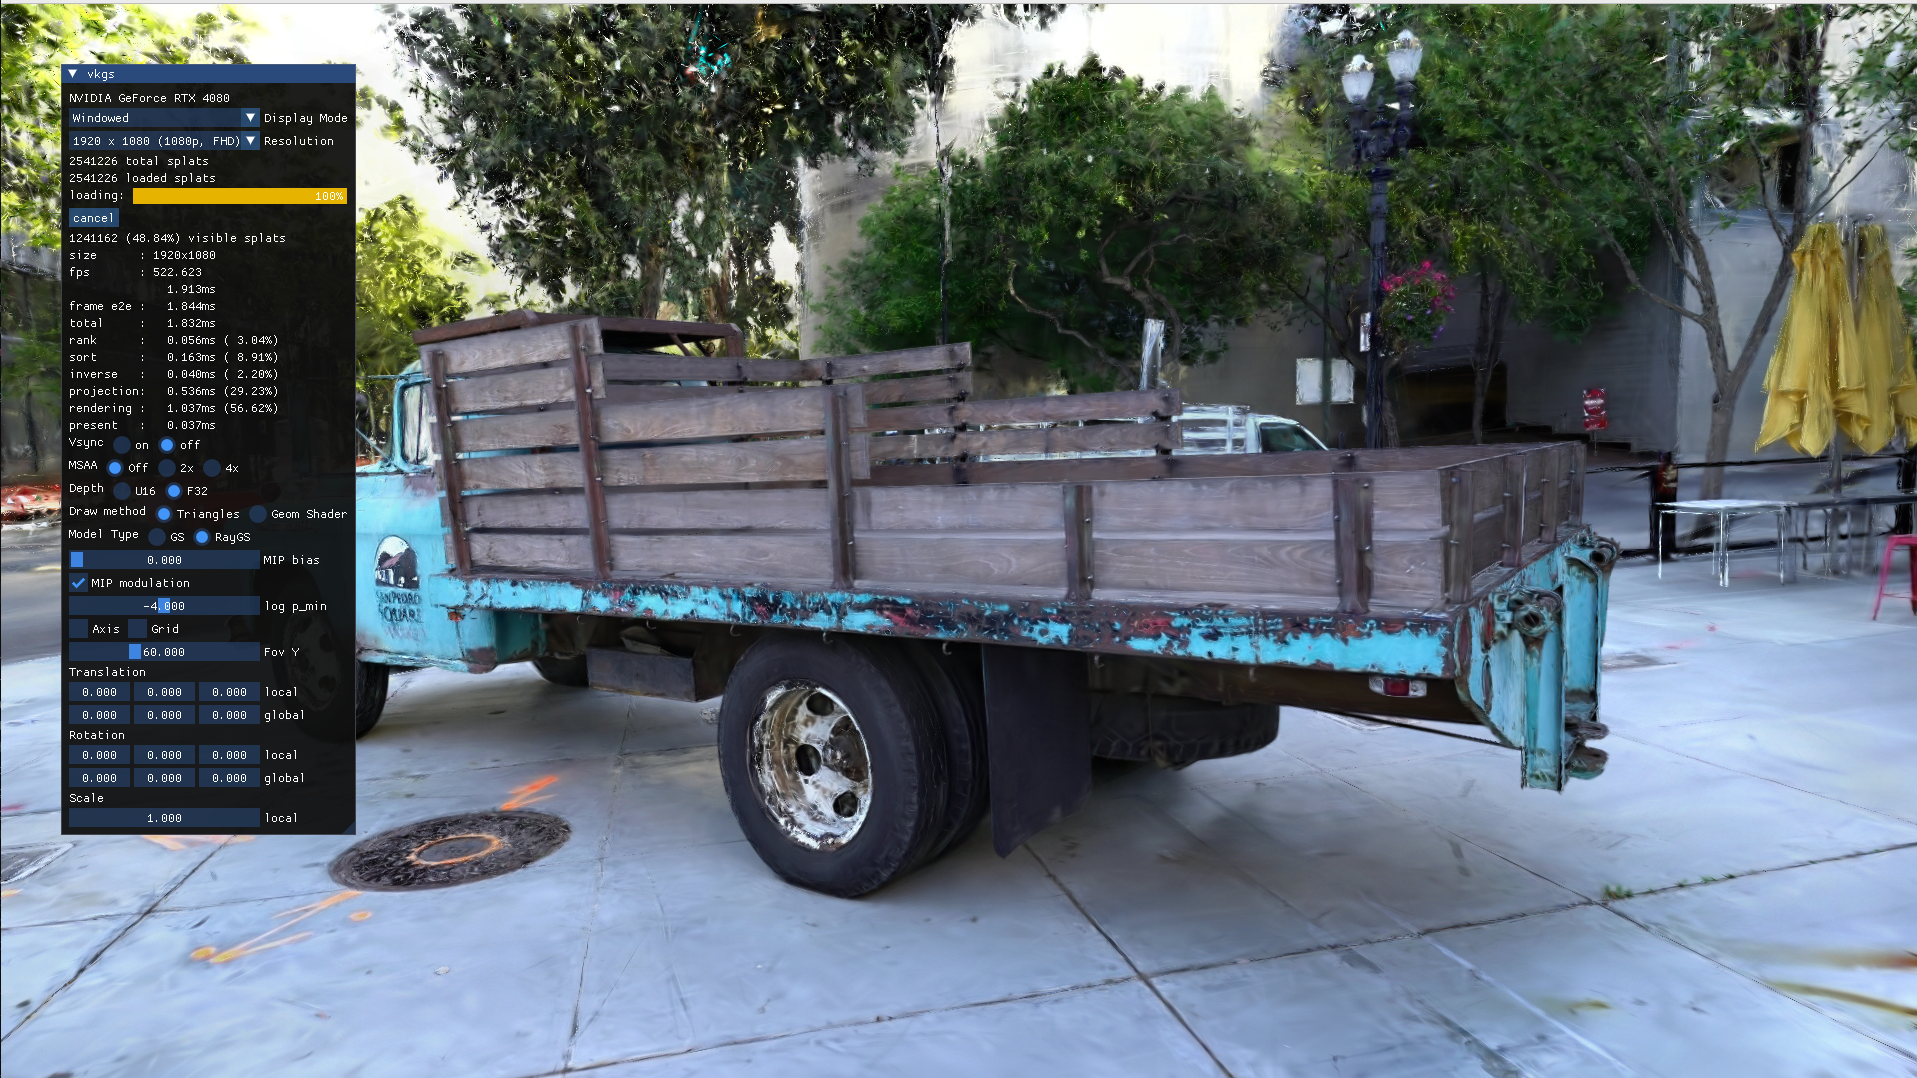
\includegraphics[width=\linewidth]{./figures/truck_cam0_raygs.png}
        \caption{\texttt{truck\_cam0\_raygs.png}}
    \end{subfigure}
    \caption{truck cam0：GS 与 RayGS 对比}
\end{figure}



\subsection{复现实验小结}
Viewer 支持鼠标旋转、平移、缩放、滚轮和 Dolly zoom，也支持分辨率、Vsync、MSAA、MIP、GS/RayGS 模式切换。由于所有测试场景均远高于 60 FPS，实际交互中相机旋转和缩放响应非常及时；在 4x MSAA 或高分辨率下仍能保持流畅，只是 GPU 利用率和功耗更高。实验记录时关闭 Vsync 可以反映算法吞吐能力，展示时打开 Vsync 则可以减少画面撕裂。

本次复现的主要成果可以概括为三点。第一，完成了基于作者预训练 Gaussian 点云和 VKRayGS Viewer 的本地测试流程，固定视角抽样、分辨率、渲染模式和日志指标，形成了可重复的 FPS、frame time、projection/rendering time、visible ratio、功耗与截图记录。第二，性能上验证了 VKRayGS 的实时交互能力：在 $1920\times1080$ 下，bicycle、garden、room、bonsai、truck 均远高于 60 FPS，其中 bonsai 和 room 等较小室内场景超过 700 FPS，garden 和 bicycle 等大规模室外场景仍保持约 400--500 FPS。第三，复现结果显示性能瓶颈并不只由 Gaussian 总数决定，还会受到当前视角可见比例、projection 阶段负载、片元填充量、分辨率和 MSAA 采样数影响；分辨率和 MSAA 增大时，rendering 阶段开销上升最明显，而 projection 时间相对稳定。



\section{综合讨论}
\subsection{本文方法的核心价值}
本文方法的核心价值在于将 RayGS 的几何一致性与硬件光栅化的高吞吐结合起来。它并没有牺牲 RayGS 的三维射线建模，而是通过三维 quad 和插值公式，把复杂的 RayGS support 计算转化为 GPU 光栅化管线擅长处理的 primitive rasterization 问题。



\subsection{性能瓶颈分析：projection、rendering 与 fill-rate}
论文和本地复现实验共同说明，性能不仅由 Gaussian 总数决定。projection 阶段更接近 primitive 数量和可见 splats 的函数；rendering 阶段则与 framebuffer 分辨率、片元覆盖面积、alpha blending、MSAA 采样数和遮挡层次有关。bicycle 和 garden 的总点数接近，但 garden 因可见比例更高而 FPS 更低；truck 总点数较少，但可见比例高，rendering 阶段耗时也较高。这些现象表明，分析 3DGS renderer 时需要同时考虑 primitive-level 和 pixel-level 两类负载。



\subsection{RayGS、MIP-RayGS 与 MSAA 的适用场景}
RayGS 更适合解决近景几何一致性问题，尤其是相机靠近物体、边缘结构复杂或自由视角移动的场景。MIP-RayGS 主要改善远景高频结构的 aliasing 和闪烁，适合辐条、树枝、围栏等小尺度细节。MSAA 对高对比轮廓有效，但性能开销更高，也不能从根本上修正 Gaussian 表达或投影近似带来的几何问题。因此，三者并不是互相替代，而是作用于不同层次的问题。



\subsection{对 VR/MR 和实时交互应用的意义}
VR/MR 场景对帧率和画质稳定性都有较高要求。传统 3DGS 的局部投影伪影在普通屏幕观看中可能不明显，但在头显、近景移动和自由交互中容易破坏沉浸感。VKRayGS 通过百级 FPS 的 RayGS 渲染，使 RayGS 模型具备进入实时交互场景的可能性。结合 MIP formulation，它也更适合处理尺度变化和远景细节闪烁问题~\cite{mipnerf360,mipsplatting}。


\subsection{仍然存在的问题与未来方向}
从论文和复现流程看，仍有若干可改进方向。论文主要加速 test-time rendering，训练阶段是否也能使用硬件光栅化仍未解决；MIP 的定量评估仍不充分；跨 GPU、跨平台和移动端表现还需要更多实验。本地复现方面，Viewer 尚未内置自动截图导出、视频导出和连续相机轨迹回放，近景运动实验仍需要人工截图和录屏。后续可以结合 3DGS 压缩、加速和动态场景工作进一步扩展，例如压缩表示、视角一致排序和动态 Gaussian 表示~\cite{lightgaussian,compressed3dgs,stopthepop,dynamic3dgaussians}，并补充开启 MIP 后的质量指标。



\section{结论}
本文围绕 \emph{Hardware-Rasterized Ray-Based Gaussian Splatting} 的方法和实验进行了整理与复现分析。传统 3DGS 渲染速度快，但依赖二维投影近似，近景时可能产生几何伪影；RayGS 几何一致性更好，但直接计算代价较高。论文发现 RayGS support 边界射线对应的最大密度点在三维空间中形成一个二维椭圆，并据此构造三维 quad，使 RayGS 能够映射到标准 GPU 光栅化管线。fragment shader 再利用硬件插值高效计算 RayGS divergence 和不透明度，从而在保持 RayGS 质量的同时获得实时帧率。

论文实验显示，VKRayGS 在 RTX2080 上相对 GOF 获得约 40$\times$ 平均加速，同时质量指标保持接近。MIP formulation 则进一步缓解远景高频结构的 aliasing。本地复现实验验证了 VKRayGS 的实时交互趋势：多个场景在 $1920\times1080$ 下均达到数百 FPS，分辨率和 MSAA 主要增加 rendering 阶段开销，RayGS 与 GS 在 FPS 接近的同时提供更稳定的近景观感。综合来看，该方法适合用于需要自由视角浏览、实时反馈和高质量几何稳定性的三维重建、数字人和沉浸式场景展示任务。



%%----------- 参考文献 -------------------%%
%在reference.bib文件中填写参考文献，此处自动生成

\reference



\end{document}